% Predlozak za pisanje diplomskog rada na PMF-MO
% Opcenita uputstva za LaTeX se mogu npr. naci na 
% http://web.math.hr/nastava/rp3, http://web.math.hr/nastava/s4-prof/latex.pdf
% NE PREPORUCA se "Ne baš tako kratak uvod u TEX", buduci se radi o vrlo starom prirucniku
% koji nije pogodan za moderne verzije LaTEXa.
% Originalna verzija "The not so short..." na http://tobi.oetiker.ch/lshort/lshort.pdf 
% je obnovljena i daje bolji uvid u moderne verzije LaTeXa

% Stil je optimiziran za kreiranje pdf dokumenta (npr. pomocu pdflatex-a, XeLaTeX-a)

\documentclass[a4paper,twoside,12pt]{memoir} % jednostrano: promijeniti twoside u oneside

% Paket inputenc omogucava direktno unosenje hrvatskih dijakritickih znakova 
% opcija utf8 za unicode (unix, linux, mac)
% opcija cp1250 za windowse
\usepackage[utf8]{inputenc}  % ukoliko se koristi XeLaTeX onda je \usepackage{xunicode}\usepackage{xltxtra}

% Stil za diplomski, unutra je ukljucena podrska za hrvatski jezik
\usepackage{diplomski}
% bibliografija na hrvatskom
\usepackage[languagenames,fixlanguage,croatian]{babelbib} % zahtijeva datoteku croatian.bdf
% hiperlinkovi 
\usepackage[pdftex]{hyperref} % ukoliko se koristi XeLaTeX onda je \usepackage[xetex]{hyperref}

% Odabir familije fontova:
% koristenjem XeLaTeX-a mogu se koristiti svi fontovi instalirani na racunalu, npr
% \defaultfontfeatures{Mapping=tex-text}
% \setmainfont[Ligatures={Common}]{Hoefler Text}
% ili
% \newcommand{\nas}[1]{\fontspec{Adobe Garamond Pro}\fontsize{24pt}{24pt}\color{Chocolate}\selectfont #1}
% i onda \nas{Naslov ...}
\usepackage{txfonts} % times new roman 

% Paket graphicx sluzi za manipuliranje grafikom 
\usepackage[pdftex]{graphicx} % ukoliko se koristi XeLaTeX onda je \usepackage[xetex]{graphicx}
% Paket amsmath je vec ukljucen
% Dodatno definirane matematicke okoline:
% teorem (okolina: thm), lema (okolina: lem), korolar (okolina: cor),
% propozicija (okolina: prop), definicija (okolina: defn), napomena (okolina: rem),
% slutnja (okolina: conj), primjer (okolina: exa), dokaz (okolina: proof)
% Definirane su naredbe za ispisivanje skupova N, Z, Q, R i C
% Definirane su naredbe za funkcije koje se u hrvatskoj notaciji oznacavaju drukcije 
% nego u americkoj: tg, ctg, ... (\tgh za tangens hiperbolni)
% Takodjer su definirane naredbe za Ker i Im (da bi se razlikovala od naredbe za imaginarni dio kompleksnog
% broja, naredba se zove \slika).



\usepackage{listings}
\usepackage{xcolor}


% \lstset{
% backgroundcolor=\color{lbcolor},
%     tabsize=4,    
% %   rulecolor=,
%     language=[GNU]C++,
%         basicstyle=\scriptsize,
%         upquote=true,
%         aboveskip={1.5\baselineskip},
%         columns=fixed,
%         showstringspaces=false,
%         extendedchars=false,
%         breaklines=true,
%         prebreak = \raisebox{0ex}[0ex][0ex]{\ensuremath{\hookleftarrow}},
%         frame=single,
%         numbers=left,
%         showtabs=false,
%         showspaces=false,
%         showstringspaces=false,
%         identifierstyle=\ttfamily,
%         keywordstyle=\color[rgb]{0,0,1},
%         commentstyle=\color[rgb]{0.026,0.112,0.095},
%         stringstyle=\color[rgb]{0.627,0.126,0.941},
%         numberstyle=\color[rgb]{0.205, 0.142, 0.73},
% %        \lstdefinestyle{C++}{language=C++,style=numbers}’.
% }
% \lstset{
%     backgroundcolor=\color{lbcolor},
%   }

\lstset { %
    language=C++,
    backgroundcolor=\color{black!5}, % set backgroundcolor
    tabsize=4,
    frame=lines,
    numbers=left,
    numberstyle=\tiny,
    numbersep=2pt,
    breaklines=true,
    showstringspaces=false,
    basicstyle=\tiny,
    keywordstyle=\color[rgb]{0,0,1},
    commentstyle=\color[RGB]{0,156,0},
    stringstyle=\color{red},
}

\addto\captionscroatian{\renewcommand{\lstlistingname}{Kod}}

\pagestyle{headings}
% uz paket fancyhdr mogu se lako kreirati fancy zaglavlja i podnozja

% Podaci koje treba unijeti
\title{OBJEKTNO ORIJENTIRANI PRISTUP METODI KONAČNIH ELEMENATA}
\author{Ivan Laković}
\advisor{prof. dr. sc. Luka Grubišić}  % obavezno s titulom (prof. dr. sc ili doc. dr. sc.)
\date{Rujan, 2018}  % oblika mjesec, godina

% Moguce je unijeti i posvetu
% Ukoliko nema posvete, dovoljno je iskomentirati/izbrisati sljedeci redak 
\dedication{Mami, tati, bratu i vama u studiju i režiji}

\begin{document}



% Naredna frontmatter generira naslovnu stranicu, stranicu za potpise povjerenstva, eventualnu posvetu i sadrzaj
% Moze se iskomentirati ukoliko nije u pitanju konacna verzija
\frontmatter

% Tekst diplomskog ...

% Diplomski rad treba poceti s uvodnim poglavljem  
\begin{intro}
Moderno strojarsko inženjerstvo (kao što je zrakoplovno, biomehaničko i automobilsko) obično koristi metodu konačnih elemenata (MKE) u dizajnu i razvoju novih proizvoda. Nekoliko modernih paketa za MKE uključuje specifične komponente poput toplinskih, elektromagnetskih, tekućih i strukturnih radnih okruženja. U strukturnoj simulaciji, MKE pomaže strahovito u proizvodnji vizualizacije krutosti i snage, kao i smanjenju težine, materijala i troškova. Osim toga samo testiranje postaje ciljano na najslabije komponente te samim time i jeftinije. \cite{wiki_fem_18} \par

Metoda konačnih elemenata numerička je metoda za rješavanje parcijalnih diferencijalnih jednadžbi koja se temelji na fizičkoj diskretizaciji kontinuuma te se koristi za rješavanje problema u inženjerstvu i fizici. Primjeri domena problema su strukturna analiza, prijenos topline, protok tekućine i slično. Početak razvoj metode konačnih elemenata se procjenjuje na četrdeset godine dvadesetog stoljeća. Za rješavanje problema potrebno je izračunati sustav velikog broja algebarskih jednadžbi što ubrzo postaje ne moguće izvesti bez pomoći kompjutera. Samim time javljaju se prvi softveri poput NASA-ino sponzoriranog NASTRAN-a koji se danas broje u desetinama pa i stotinama. Za razliku od prvih softvera današnji se većinom baziraju na programskom jeziku C++ koji je nastao 1985. radi njegove brzine i podrške objektno orijentiranom programiranju. Osim toga većina modernih programa nudi i grafičko sučelje (Autodesk Simulation), ali i programsko sučelje prema višim programskim jezicima poput Python-a, Ruby-a, Julia-e čime se pokušava postići apstrakcija između softvera za rješavanje i specifičnog problema potrebnog za riješiti. \cite{wiki_list_of_fem_software} \par

U ranim 1990-tim objektno orijentirano programiranje (OOP) postaje dominantna programerska paradigma obećavajući mogućnost ponovne upotrebe komponenata i proširenje postojećih putem nasljeđivanja, motivirana rastućoj popularnosti grafičkih korisničkih sučelja. OOP je bazirano na konceptu "objekata" koji najčešće sadrže podatke, te metodama koje izvršavaju neke procedure nad objektima. Samim time gotovo svi softveri za rješavanje problema metode konačnih elemenata nakon toga se razvijaju pomoću objektno orijentirane paradigme koja uvelike olakšava proširenje generalnih značajkih programa na specifične zahtjeve ne toliko raširenih domena. To dovodi do daljnjeg rasta softvera za rješavanje metode konačnih elemenata koji danas obuhvaćaju raznolike probleme i domene.  \par

U ovom radu opisat ćemo OOFEM koji je jedan takav alat, kako ga koristiti pomoću Python-a i komandne linije, te kako mu dodati nove značajke. OOFEM koji je akronim za Object Oriented Finite Element Method je softver za rješavanje problema metode konačnih elemenata razvijen s GNU General Public License što omogućava njegovu slobodnu primjenu i modifikaciju čak i u komercijalne svrhe. Borek Patzak je  započeo razvoj OOFEM-a 1993. godine, te je još uvijek vodeća osoba na projektu i dan danas nadograđuje softver. \par

Rad se sastoji od 3 poglavlja. Nakon Uvoda, u Poglavlju 1 predstavljamo metodu konačnih elemenata gdje će se ukratko opisati najvažnija svojstva potrebna za razumijevanje korištenja softvera za njezino rješavanje. Poglavlje 2 opisuje OOFEM. U njemu će biti predstavljeno što program očekuje kao ulaz, kako ga proširiti u slučaju nepostojanja traženih značajki te njegovo upravljanje putem Python programskog jezika. Također biti će objašnjeno što izlazni podaci znače te kako ih vizualizirati radi jasnije interpretacije rezultata. U trećem poglavlju pokazat ćemo na testnom primjeru kako izgleda učitavanje podatak, izračunavanje, te vizualizacija dobivenih rezultata.

\end{intro}


\chapter{Metoda konačnih elemenata}	
U ovom poglavlju cilj nam je objasniti ključne pojmove vezane uz metodu konačnih elemenata potrebne za razumijevanje računarskih alata za njihovo računanje tako da se njihovo korištenje ne svede samo na "crnu kutiju" kojoj se da ulaz i ona vrati slike. Za početak dat ćemo kratki povijesni uvod. Nakon uvoda radi lakšeg snalaženja opisati ćemo nekoliko konačnih elemenata. Nakon toga, radi motivacije ukratko ćemo objasniti fizikalne poveznice s matematičkom pozadinom što će nam dati bolju intuiciju o samim podacima. Za kraj, pokazat ćemo na jednostavnom primjeru kako bi se ručno riješio problem pomoću metode konačnih elemenata. Radi jednostavnosti i povezanošću s temom rada ograničili smo se samo na probleme mehanike deformabilnih tijela u elastičnom području. Ovo poglavlje se temelji na \cite{jurica_soric}, \cite{coursera} i \cite{wiki_fem_18}.

\section{Razvoj metode konačnih elemenata}
Iako točan datum izuma metode konačnih elemenata nije poznat, postupak je nastao iz potrebe za rješavanjem složenih problema iz područja elastičnosti i strukturne analize u civilnom i aeronautičkom inženjerstvu. A. Hrennikoff je 1941. godine pokušao riješiti problem teorije elastičnosti pri čemu je na temelju intuicije elastični kontimuum podijelio na više jednostavnih međusobno spojenih štapnih elemenata. Na taj je način kontinuirani sustav zamijenio rešetkastom konstrukcijom za koju je bilo moguće naći rješenje pomoću tada već poznatih standardnih metoda. U Kini, u kasnijim pedesetim i početkom šezdesetih godina, na temelju izračuna konstrukcija brane K. Feng predložio je sustavnu numeričku metodu za rješavanje parcijalnih diferencijalnih jednadžbi. Metoda je nazvana metodom konačnih razlika temeljenih na načelu varijacije, što je bio još neovisni izum metode konačnih elemenata. Iako su ovi pristupi različiti, oni dijele jednu bitnu karakteristiku koja je nadalje postala okosnica metode konačnih elemenata, a to je mrežna diskretizacija kontinuirane domene u skupinu diskretnih poddomena, obično nazvanih elemenata. A. Hrennikoff diskretizira domenu pomoću analogije rešetke, dok R. Courant uzima pristup tako da dijeli domenu u konačne trokutaste podregije za rješavanje eliptičnih parcijalnih diferencijalnih jednadžbi (PDE) drugog reda koji proizlaze iz problema torzije cilindra. Courantov je doprinos bio evolucijski, na temelju velikog broja prethodnih rezultata za PDE koje su razvili Rayleigh, Ritz i Galerkin. \cite{wiki_fem_4} \cite{wiki_fem_5} \par

Podjela elastičnog kontinuuma na više elemenata, koji čine manje dijelove kontinuuma koji se spajaju u zajedničkim točkama, prvi se put pojavljuje u radovima J. H. Argzrisa 1954. goidne i M. J. Turnera, R. W. Clouga, H.C. Martina i L.J. Toppa 1956. godine. Metoda konačnih elemenata dobila je pravi poticaj 1960-ih i 1970-ih godina. Matričnim zapisom u metodama analize konstrukcija omogućava primjenu na računalima što daje dodatni poticaj za daljnji razvoj. To je najbolje vidljivo iz broja publikacija iz metode konačnih elemenata koji naglo raste. Prema \cite{jurica_soric_117}, broj radova je s 10 i 15 1961. godine i 1962. godine narastao na 162 rada 1967. godine te na 303 rada 1968. godine. Rast popularnosti metode konačnih elemenata dobro se vidi iz idućeg grafa s brojem publikacija po godini.
\begin{figure}[h!t]
\begin{center}
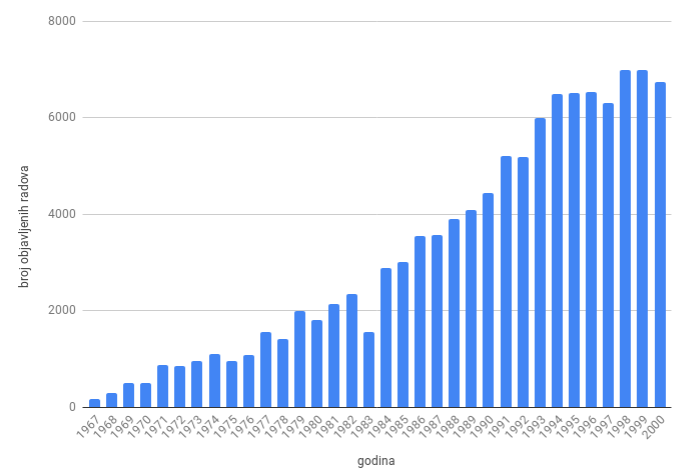
\includegraphics[scale=0.5]{pictures/chapter_fem/broj_objavljenih_radova.png}
\caption{Pregled objavljene literature iz metode konačnih elemenata za razdoblje 1967.-2000. \cite{jurica_soric_76}}
\end{center}
\end{figure}
Paralelno s time rastao je i broj dostupnih softverskih programa. Tako su Abaqus, Adina, Ansys, i drugi softverski paketi nastali već 1970-tih godina od kojih se mnogi i dan danas koriste. Još jedan od ključnih razloga za strmoglavi rast popularnosti je to što se metoda konačnih elemenata počela primjenjivati ne samo u strukturnoj analizi već i u analizi fluida, prijenosu topline, elektrostatičkim problemima i još brojim drugim područjima. \par

Danas su strojarstvo, brodogradnja, zrakoplovstvo, automobilska industrija i građevina nezamislivi bez metode konačnih elemenata koja im pomaže u različitim pogledima čineći krajnji proizvod bolji i jeftiniji. Rastom računalne snage računala te modernog računanja na grafičkim karticama metoda konačnih elemenata može lagano rukovati s vrlo složenim geometrijama što je izdvaja iznad ostalih metoda. Važne značajke su također i to što može obraditi složena ograničenja na rubne uvjete i opterećenja poput pritiska, temperature i inicijalnih sila.
\begin{figure}[h!t]
\begin{center}
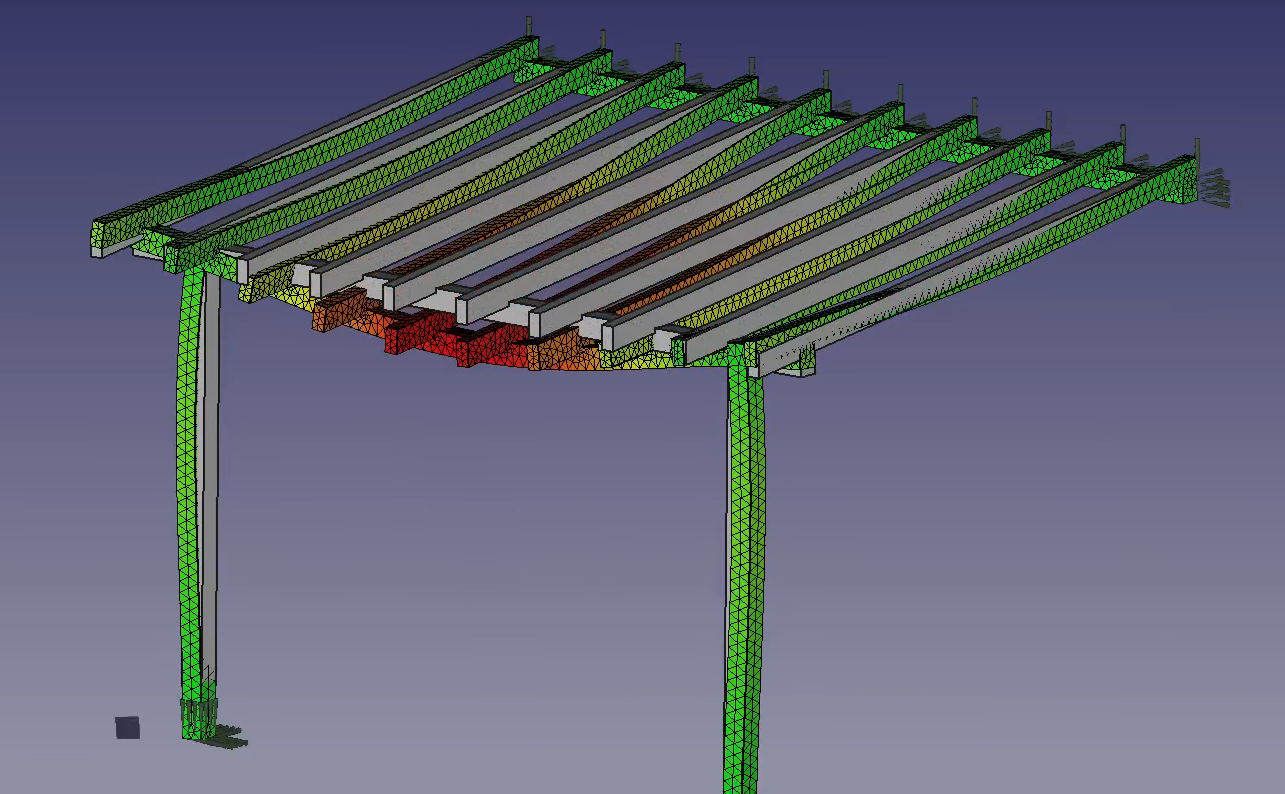
\includegraphics[scale=0.3]{pictures/chapter_fem/FEM_primjer.png}
\caption{Primjer analize problema nadstrešnice u softverskom alatu FreeCAD \cite{youtube_freecad}}
\end{center}
\end{figure}


\section{Osnovni konačni elementi i njihova primjena}
Kako je metoda konačnih elemenata numerička metoda koja kontinuum s beskonačno stupnjeva slobode gibanja zamjenjuje s diskretnim modelom međusobno povezanih elemenata postavlja se pitanje kakvi su ti elementi te kakvi sve mogu biti. Ovisno o obliku i nepoznatim parametrima u čvorovima izvedeni su različiti tipovi konačnih elemenata. Veći broj nepoznanica zahtjeva složeniju interpolacijsku funkciju u području elemenata. Jednostavniji konačni elementi koji se najčešće primjenjuju u mehanici deformabilnih tijela prikazani su na idućoj slici. Nepoznati parametri u čvorovima, koji u metodi pomaka u mehanici deformabilnih tijela opisuju pomake i derivacije pomaka, stupnjevi su slobode elemenata. \par

Za linearne funkcije u 2D i 3D, najčešći su elementi prikazani na slici \ref{fig:2d_i_3d_elementi}. Pomoću konačnih elementa za dvodimenzijsku analizu prikazanih na slici moguće je opisati ravninsko stanje naprezanja i deformacije pri čemu su nepoznati parametri u čvorovima dvije komponente pomaka. U 2D, pravokutni elementi se često primjenjuju na analize strukturalnih mehanika. Također se mogu koristiti za granični sloj umrežavanja u računalnoj dinamici fluida i modeliranju toplinskog prijenosa. Elementi za trodimenzijsku analizu s čvorovima sa po tri komponente pomaka u pravcu Kartezijevih koordinatnih osi koji su analogija 2D elemenata poznati su kao heksadedarski elementi i obično se primjenjuju na strukturalnu mehaniku i umrežavanje graničnog sloja. U prijelazu iz heksadedrijskih elemenata graničnog sloja na tetraedarske elemente, piramidalni elementi obično se postavljaju na vrh elementa graničnog sloja.

\begin{figure}[h!t]
\begin{center}
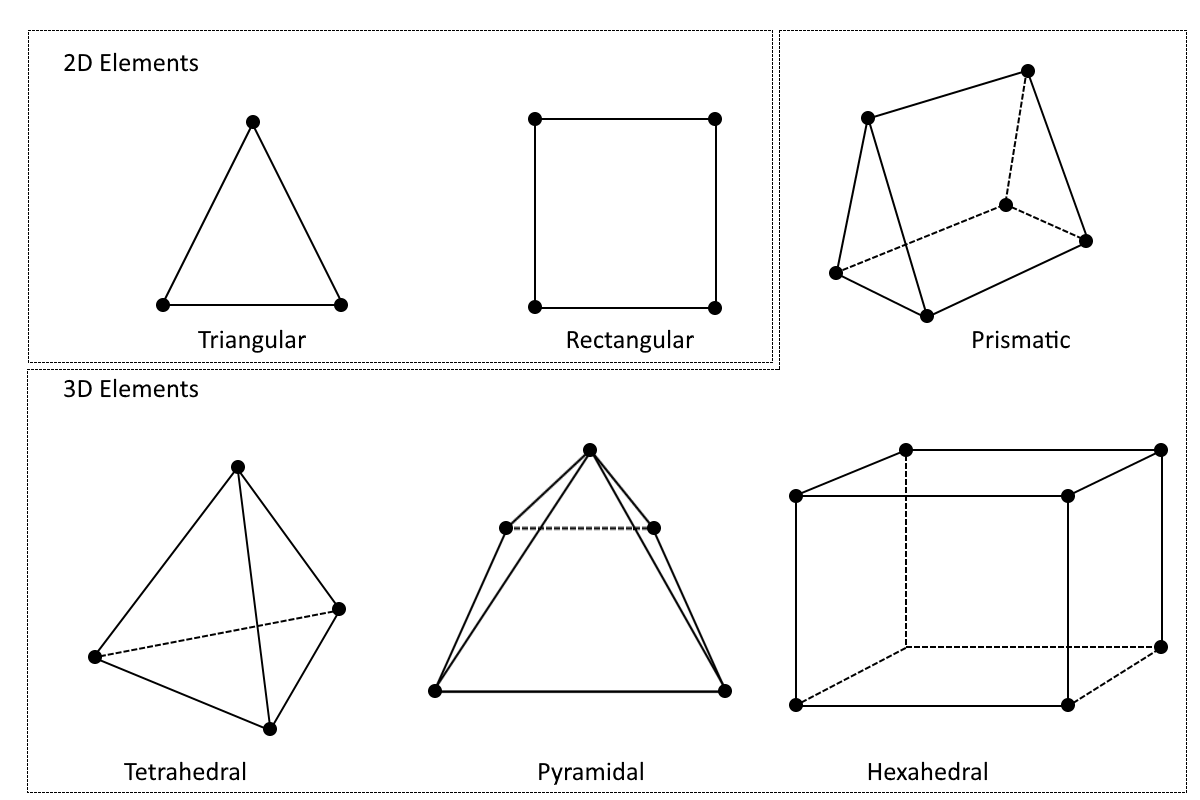
\includegraphics[scale=0.47]{pictures/chapter_fem/geometry-and-nodes-linear-elements.png}
\caption{Položaj čvorova i geometrija za 2D i 3D linearne elemente. \cite{comsol_fem_general}}
\label{fig:2d_i_3d_elementi}
\end{center}
\end{figure}

Na slici \ref{fig:base_triangle_elements} prikazane su funkcije s linearnom osnovom koje definiraju trokutastu mrežu koja je sastavljena od trokutastih linearnih elementa. Temeljne funkcije izražene su kao funkcije položaja čvorova ($x$ i $y$ u 2D i $x$, $y$ i $z$ u 3D).

\begin{figure}[h!t]
\begin{center}
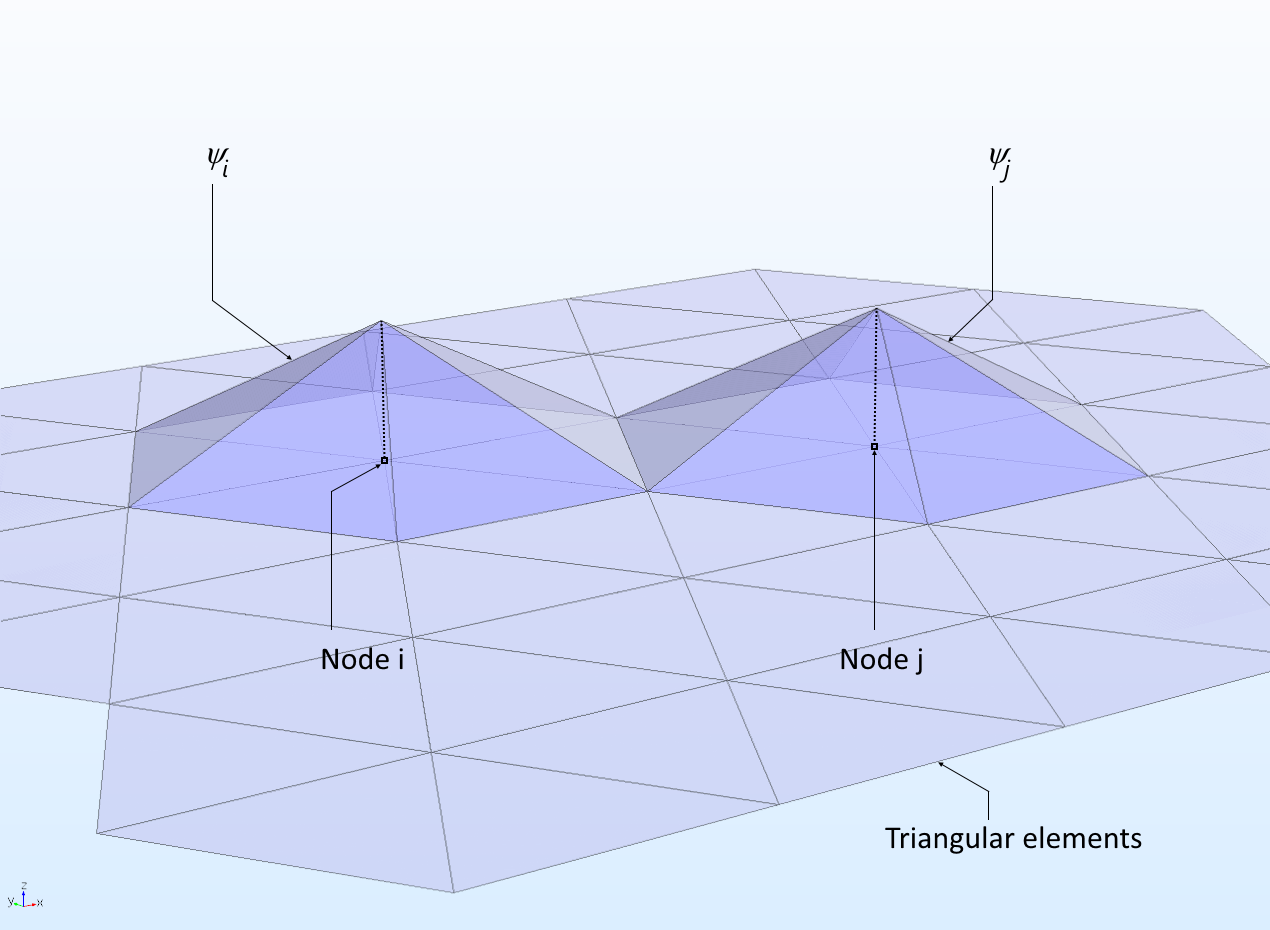
\includegraphics[scale=0.42]{pictures/chapter_fem/base-functions-no-overlap.png}
\caption{Dvije osnovne funkcije koje dijele jedan element vrh, ali se ne preklapaju u 2D domeni. \cite{comsol_fem_general}}
\label{fig:base_triangle_elements}
\end{center}
\end{figure}

\par
U praksi objekti koje je potrebno modelirati su ne rijetko složeniji te samim time zahtijevaju i složenije konačne elemente. Jedan primjer je element za analizu ljusaka sa šest stupnjeva slobode (položaj čvorova u $x$, $y$ i $z$ osi te rotacije po tim osima) a izvodi se superpozicijom osnovnog pločastog elementa i elementa za dvodimenzijsku analizu. Postoje i složeniji dvostruko zakrivljeni ljuskasti elementi koji u čvorovima mogu imati i znatno više stupnjeva slobode. Također, svaki od prikazanih elementa moguće je proširiti dodavanjem čvorova duž bridova ili po površini elementa. \par

Nadalje dajmo 2 primjera različitih konstrukcija podijeljenih na konačne elemente na koje su primijenjeni elementi iz gornjeg dijela. Na slici \ref{fig:mesh_rim} dajemo primjer podjele naplatka kotača na konačne elemente. Lijeva podjela sastoji se samo od tetraedara kojih ima oko 145,000 s oko 730,000 stupnjeva slobode, dok je desna sastavljena od tetraedara (zeleni), kvadara (plavi) i prizmi (rozi). Desna podjela ima oko 78,000 elemenata i nešto manje od 414,000 stupnjeva slobode što ju čini gotovo dvostruko manjom od lijeve. Na idućoj slici, slika \ref{fig:mesh_spring} imamo dvije različite podjele opterećene opruge na konačne elemente koristeći samo prizme odnosno tetraedre. Dok mreža s prizmama ima oko 504 elemenata i 9526 stupnja slobode, mreža s tetraedrima ima 3652 tetraedra i 23,434 stupnja slobode.

\begin{figure}[h!t]
\begin{center}
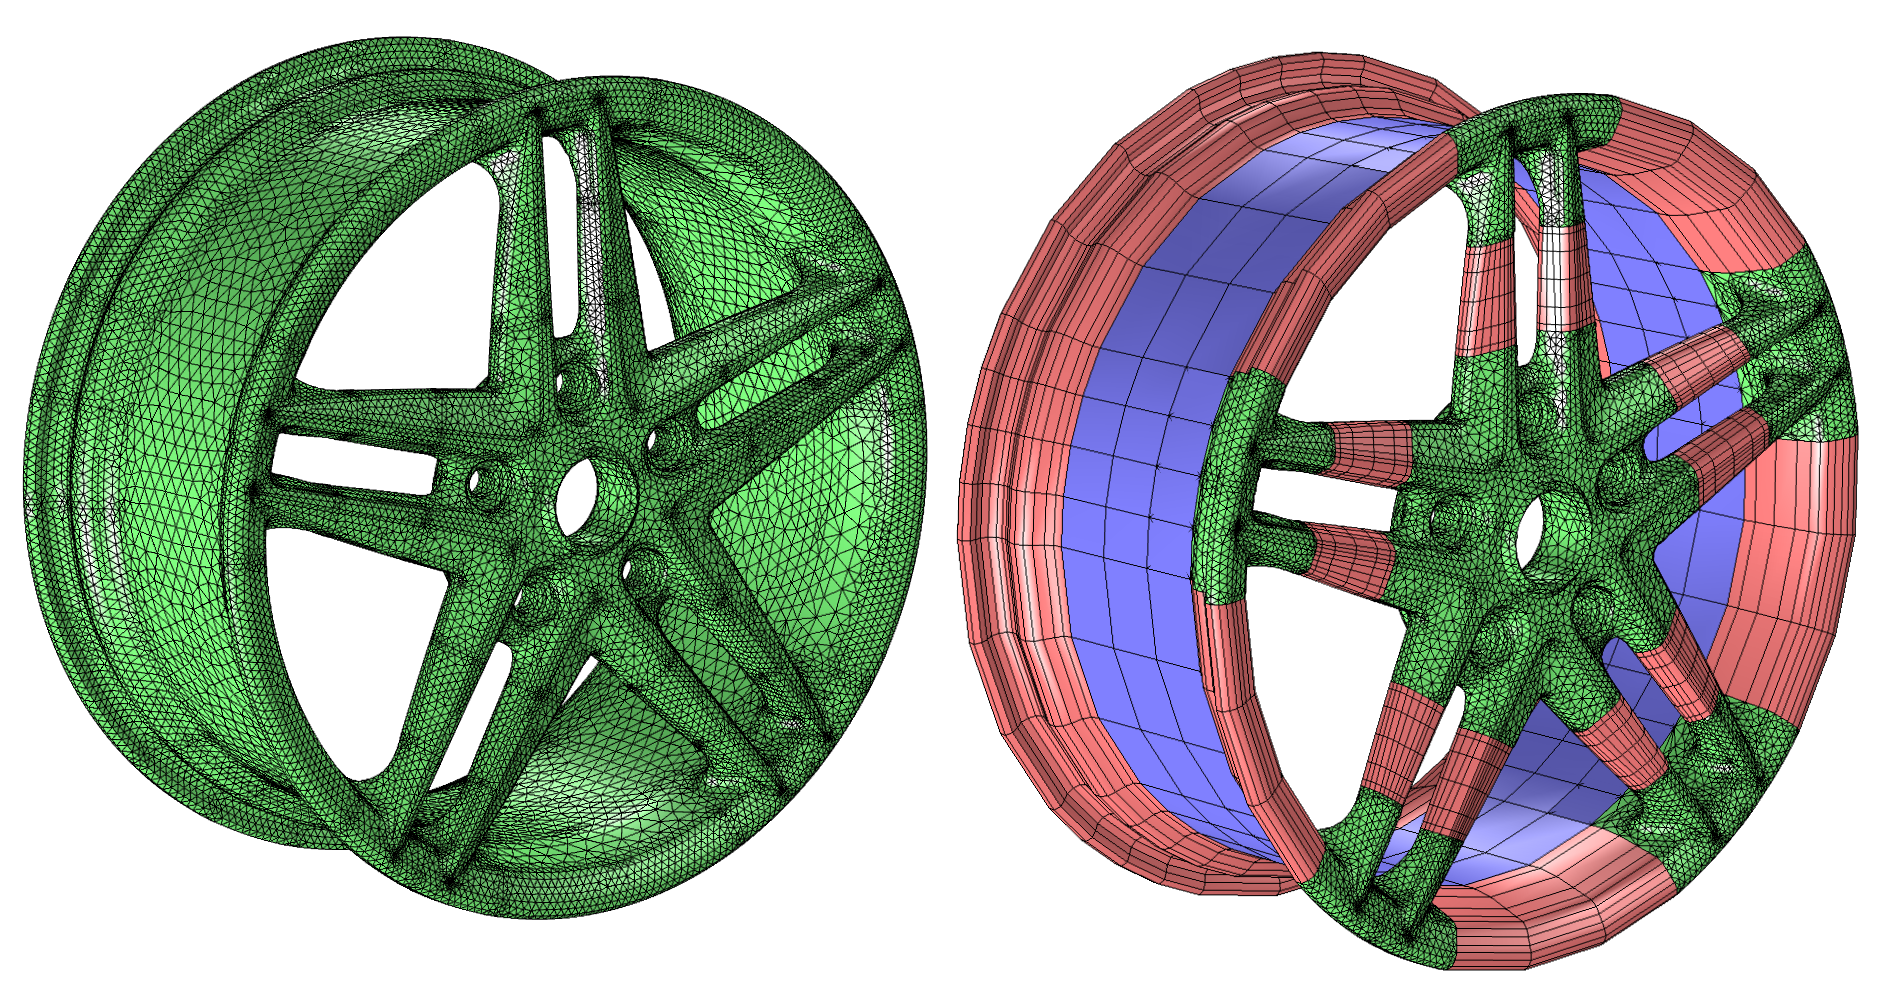
\includegraphics[scale=0.2]{pictures/chapter_fem/Wheel-rim-mesh-example-large.png}
\caption{Primjer mrežastog modela automobilskog naplatka \cite{comslo_mesh}}
\label{fig:mesh_rim}
\end{center}
\end{figure}

\begin{figure}[h!t]
\begin{center}
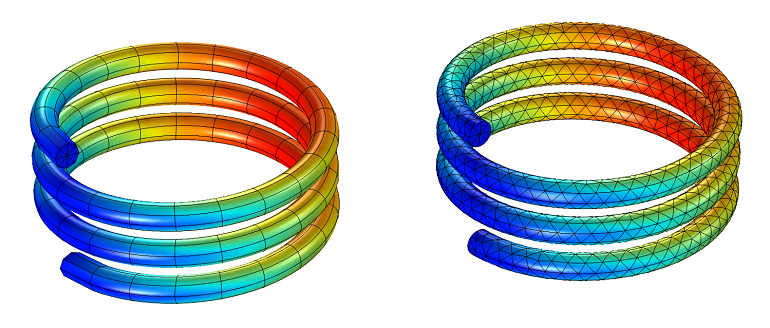
\includegraphics[scale=0.6]{pictures/chapter_fem/Loaded-spring-example.png}
\caption{Primjer mrežastog modela opterećene opruge \cite{comslo_mesh}}
\label{fig:mesh_spring}
\end{center}
\end{figure}

\par
Kao što je vidljivo iz gornjih slika čak i za relativno jednostavne konstrukcije mreža brzo postaje prevelika za analognu izradu stoga se oslanjamo na softverske programe za njihovu izradu. Što se samog postupka tiče postoji mnogo različitih pristupa izradi mrežastog modela, ali klasifikaciju mreže možemo podijeliti na strukturiranu mrežu, ne strukturiranu te hibridnu koja uzima prednosti svake od nje. Postoji mnogo alata koji služe za pretvaranje modela izrađenih u softverima poput CAD-a, NURBS-a, STL-a u mrežasti model. Neki od popularnijih su GMSH, ICEM, Gridgen. Popularni komercijalni softveri za rješavanje problema pomoću metode konačnih elemenata ujedinjuju dizajniranje modela, pretvorbu modela u mrežasti te računanje metodom konačnih elemenata. Također, radi postizanja točnijih rezultata i manje greške koristi se i h/p-metoda koja mijenja veličinu i stupnjeve slobode elemenata te tako povećava preciznost izračuna na mreži nakon računanja metode konačnih elemenata u kritičnim područjima. Tako dolazimo do iterativnog postupka generiranja mreže koji svakom iteracijom postaje profinjeniji te samim time i točniji. \par 

U ovom radu naglasak je na postupak nakon dobivene mreže stoga se neće ići u dubinu njezine izrade. Više o izradi mreže može se naći u \cite{tadej}

\section{Računanje metode konačnih elemenata}
Ovo potpoglavlje temelji se na \cite{jurica_soric} i \cite{fem_predavanja_bosna} te pokazuje što je sve potrebno prilikom rješavanja problema metodom konačnih elemenata.
Postoje dva osnovna pristupa metodi konačnih elemenata. 
Prva je metoda sila (metoda fleksibilnosti). U metodi sila osnovne nepoznate veličine u problemu koji se analiziraju su sile. Da bi se dobile jednadžbe strukture, prvo se postavljaju jednadžbe ravnoteže. Rezultat je sustav algebarskih jednadžbi u kojima se nepoznate veličine sile određuju iz jednadžbi.
Drugi pristup je metoda pomicanja (metoda krutosti) u kojoj postoje osnovna nepoznata kretanja u čvorovima. Kako bi se postigli uvjeti kompatibilnosti za rješavanje specifičnih problema, potrebno je da su elementi povezani u čvorovima, uz stranice ili odgovarajuće površine prije i nakon opterećenja. Jednadžbe strukture sadrže pomicanje čvora i koriste se jednadžbe ravnoteže i odnos između sile i pomaka. 
Od dva gore spomenuta pristupa, popularnija je druga metoda, metoda pomaka. Formulacija metode pomaka slična je mnogim strukturnim problemima. Većina softverskih programa se temelji na metodama kretanja. \par

Nakon što se konstruira mreža međusobno povezanih konačnih elemenata, svakom se elementu pridružuje funkcija pomaka. Svi elementi su izravno ili neizravno povezani, uključujući čvorove i/ili zajedničke granične linije elemenata i/ili zajedničke površine.
Na temelju poznatih vrijednosti napona i deformacije u jednom čvoru i elementu, moguće je odrediti naprezanja i deformacije za bilo koji drugi čvor i element strukture koja se razmatra i čija su svojstva materijala i opterećenja već poznati. Ukupni broj strukturnih jednadžbi opisuje ponašanje svih čvorova i predstavlja sustav algebarskih jednadžbi koji je najbolje zapisan u obliku matrice \par

Prvi korak nakon diskretizacije domene na konačne elemente je izbor funkcije pomaka. Izbor funkcije pomaka obavlja se za svaki element. Funkcija je definirana unutar elementa i koristi vrijednosti izračunate u čvorovima. Za funkcije pomaka najčešće se izabiru linearni, kvadratni ili kubni polinomi. Polinomi se koriste kao funkcije jer su jednostavni za računanje metode konačnih elemenata. Za dvodimenzionalni element, funkcija pomaka je funkcija koordinata u $xy$ ravnini. Funkcije su nepoznate veličine u čvorovima. Za dvodimenzionalne probleme nepoznate veličine su funkcije koordinata $x$ i $y$.
Ista funkcija pomaka može se odabrati za svaki element u modelu konačnih elemenata diskretne strukture. Odabrane su funkcije kako bi se postigao kontinuitet pomaka u tijelu korištenjem metode konačnih elemenata između svih elemenata u čvorovima, duž stranica i površine. Nakon odabira funkcije pomaka, uspostavlja se veza između deformacija i pomaka, kao i veza između naprezanja i deformacije. \par

Nadalje, potrebno je uspostaviti vezu između deformacije i pomaka (kinematičke relacije) te vezu između naprezanja i deformacije (konstitutivne jednadžbe). Ukoliko se ograničimo na jednodimenzionalan problem tada postoji deformacija samo u jednom pravcu (pravac $x$). Tada je deformacija $\epsilon_x$ i ona je povezana sa pomakom $u$ u $x$ pravcu. Veza između pomaka i deformacije dana je jednadžbom
\begin{equation}
    \label{eq:veza_pomaka_deformacije}
	\epsilon_x = \frac{du}{dx}
\end{equation}
Jednadžba vrijedi za male deformacije i pomake. Jedna od najjednostavnijih konstitutivnih jednadžbi između deformacije i naprezanja je relacija koja se zove Hooke-ov zakon. Za jednodimenzionalni problem veza naprezanja i deformacije je 
\begin{equation}
    \label{eq:veza_naprezanja_deformacije}
    \sigma_x = E * \epsilon_x
\end{equation}
gdje je $\epsilon_x$ naprezanje u pravcu $x$, a $E$ modul elastičnosti. \par

Pomoću prethodnih relacija konstruira se matrica krutosti. U početku, matrice krutosti elemenata i jednadžba elemenata određivane su pomoću koeficijenata krutosti, što je izravno povezano sa strukturnom analizom. Nakon toga razvijeno je nekoliko metoda za određivanje matrice krutosti.
\begin{enumerate}
    \item Direktan postupak konačnih elemenata (Direct Finite Element Method) -
    Matrica krutosti povezuje sile u čvorovima elemenata i pomake čvorova. Dobiva se iz ravnotežnih uvjeta za svaki razmatrani element. Izravni pristup računanju matrice krutosti je dobar samo u slučaju jednodimenzionalnih (štapnih) elemenata, međutim, vrlo je prikladan za objašnjenje osnovnog koncepta metode konačnih elemenata.
    
    \item Varijacijski prnicipi (Variational Finite Element Methods) -
    Prilikom rješavanja složenijih, dvodimenzijskih i trodimenzijskih problema teorije elastičnosti, teško je u potpunosti zadovoljiti osnovne relacije konačnih elemenata. To je razlog za primjenu varijacijskih principa u kojima su sadržane relacije teorije elastičnosti pomoću kojih je, uz dopuštenu grešku, moguće provesti približno rješavanje problema. Na taj su način i odgovarajuće jednadžbe teorije elastičnosti približno zadovoljene. Primjer varijacijskih principa su principi virtualnih pomaka i virtualnih sila koji su za rješavanje problema mehanike deformabilnih tijela u elastičnom području ekvivalentni principima minimuma potencijalne energije.
    
    \item Metoda težninskog reziduala (Methods of Weighted Residuals) -
    Ova se metoda temelji na diferencijalnim jednadžbama razmatranog problema. Metoda se koristi kada nije moguće utvrditi funkcional i za probleme u kojima funkcional uopće ne postoji. Od svih metoda težniskog reziduala najpoznatija je Galerkinova metoda. Na temelju metode reziduala dobivene su jednadžbe koje opisuju ponašanje elemenata. U matričnom obliku to izgleda:
    $$
    \begin{pmatrix} f_1 \\ f_2 \\ \vdots \\ f_n \end{pmatrix}
    =
    \begin{bmatrix}
    k_{11}       & k_{12} & k_{13} & \dots & k_{1n} \\
    k_{21}       & k_{22} & k_{23} & \dots & k_{2n} \\
    k_{n1}       & k_{n2} & k_{n3} & \dots & k_{nn}
    \end{bmatrix} 
    \begin{pmatrix} d_1 \\ d_2 \\ \vdots \\ d_n \end{pmatrix}
    $$
    $$ f = K * d $$
    gdje su: \\
    $f$ vektor sila u čvorovima elementa \\
    $K$ matrica krutosti elemenata \\
    $d$ vektor pomaka čvorova elemenata 
\end{enumerate}
Osim navedenih postoji još metoda poput Razleigh-Ritzova metode i metode energetske ravnoteže koje nećemo detaljnije opisivati. Korištenjem neke od gore navedenih metoda dobiju se matrice krutosti i jednadžbe pojedinih konačnih elemenata te je kao idući korak potrebno izračunati globalnu matricu krutosti. \par

Primjenom metode direktne superpozicije (Direct Stiffness Method), jedne od metoda koja se danas najčešće primjenjuje za izvođenje globalne jednadžbe konačnih elemenata i globalne matrice krutosti, matrice pojedinih elemenata se kombiniraju. Prilikom primjene metode mora se poštivati koncept kontinuiteta ili kompatibilnosti, što zahtijeva da struktura zadržava cjelovitost to jest, ne smije doći do prekida strukture. Globalna jednadžba strukture u obliku matrice je:
\begin{equation}
\label{eq:glob_jed_strukture}
	F = K * d
\end{equation}
gdje su: \\
$f$ vektor opterećenja u globalnom koordinatnom sustavu \\
$K$ globalna matrica krutosti \\
$d$ vektor poznatih i nepoznatih pomaka svih čvorova strukture \\

Globalna matrica krutosti $K$ je simetrična i singularna matrica. Problem singulariteta matrice rješava se uvođenjem rubnih uvjeta tako da struktura zadrži postojeće mjesto i da se ne kreće kao kruto tijelo. Tako matrica krutosti postaje pozitivno definitna što je uvjet za mogućnost rješavanja nehomogenog sustava jednadžbi.
Formiranje globalne matrice krutosti danas se u računalu najčešče provodi takozvanim postupkom popunjavanja, pri čemu se kinematička matrica transformacije zamjenjuje tablicom iz koje je vidljivo koji lokalni stupnjevi slobode odgovaraju globalnim stupnjevima slobode. Počinje se s nul-matricom te se nadalje popunjava. \par

Rješavanjem gornje jednadžbe matrične strukture (\ref{eq:glob_jed_strukture}) u koju su uneseni rubni uvjeti dobivamo vrijednosti globalnog vektora pomaka $d$. Rješavanje sustava se provodi Gausovom metodom eliminacije ili primjenom neke od iterativinih metoda. Nepoznanice koje se dobiju rješavanjem su pomaci u čvorovima. To su prvi rezultati koji se dobiju primjenom metode konačnih elemenata. \par

Nakon rješavanja globalnog sustava jednadžbi i izračunavanja globalnog vektora pomaka $d$, potrebno je izračunati naprezanje u konačnim elementima. Za dobivanje tih vrijednosti koristimo veze između deformacija, naprezanja i pomaka iz (\ref{eq:veza_pomaka_deformacije}) i (\ref{eq:veza_naprezanja_deformacije}). Pomoću navedenih izraza moguće je odrediti naprezanje u proizvoljnoj točki konačnog elementa. Naprezanja se izračunavanju u težištu elementa, u čvorovima ili u točkama numeričke integracije. Važno je naglasiti da se pri gruboj diskretizaciji mogu naprezanja po rubovima susjednih elemenata znatno razlikovati, odnosno naprezanja koja pripadaju različitim susjednim elementima duž zajedničkog ruba mogu biti različitog iznosa. Razlike se mogu smanjiti usitnjavanjem mreže konačnih elemenata. U slučaju različitih vrijednosti duž rubova, za procjenu stanja naprezanja izračunava se srednja vrijednost. \par

Rezultati dobiveni primjenom metode konačnih elemenata se interpretiraju tako da se odrede mjesta djelovanja najvećih naprezanja i deformacija. Na temelju znanja o materijalima i strukturi tada inženjer donosi daljnje odluke mora li se, i želi li se dizajn strukture mijenjati te se ovisno o odgovoru postupak ponavlja. Računalni programi za naknadnu obradu (vizualizaciju) pomažu inženjerima analizu izradom toplinskih karata "heat map" tako da se dijelovi strukture s većim naprezanjima/deformacijama bojaju u toplije a područja s manjim u hladnije boje. Velik broj softverskih alata za rješavanje metode konačnih elemenata dolazi s ugrađenim softverom za vizualizaciju stoga se iteriranje modela postaje prirodan tok dizajniranja novih struktura.

\begin{figure}[h!t]
\begin{center}
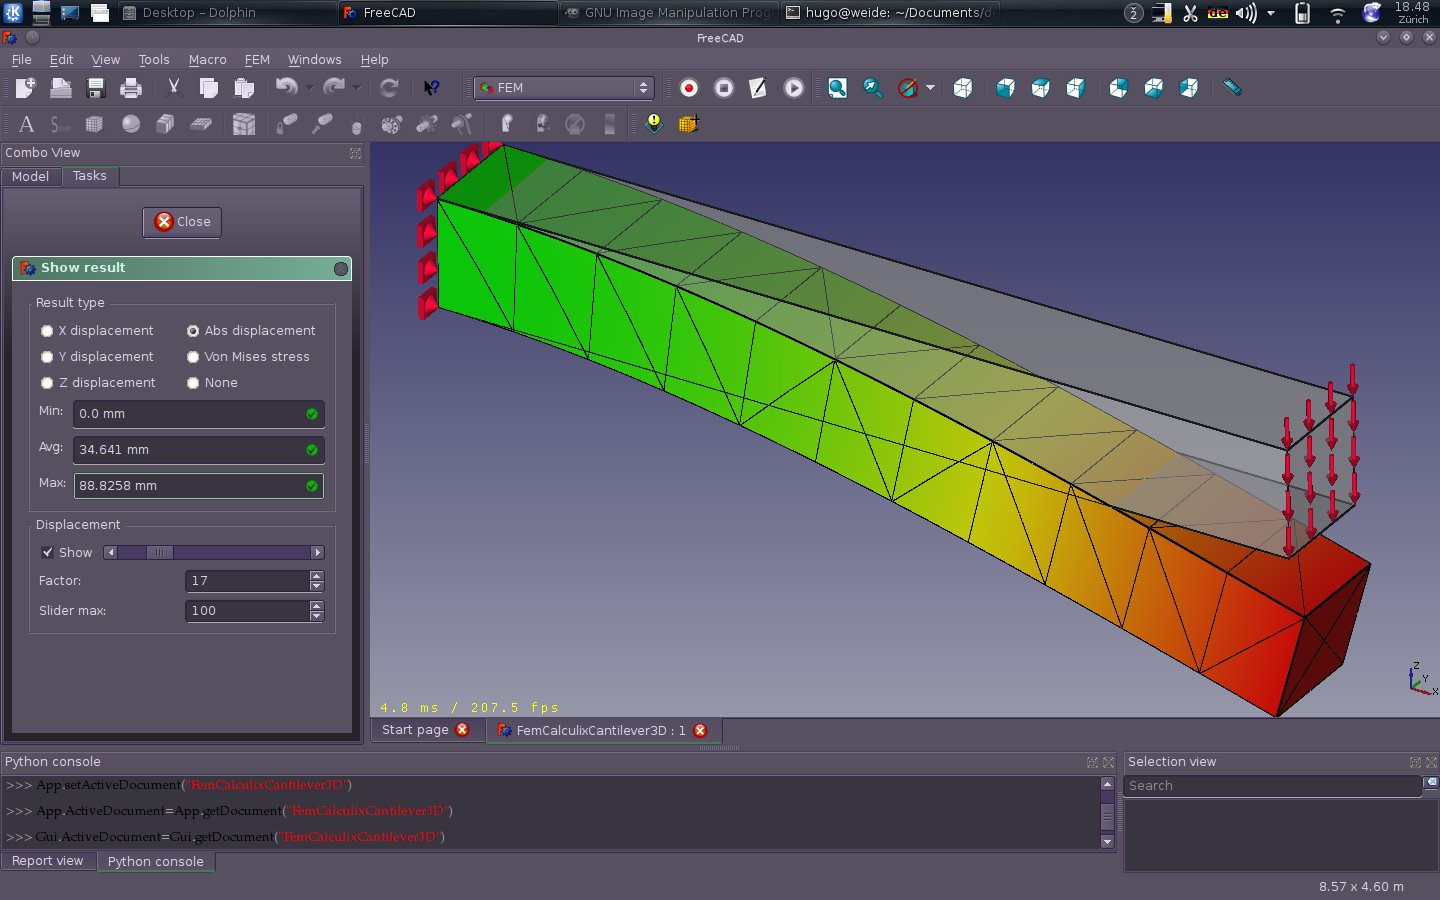
\includegraphics[scale=0.35]{pictures/chapter_fem/FEM_visualization_1.jpg}
\caption{Primjer vizualizacije opterećenja na gredu u softverskom alatu FreeCAD \cite{freefem_wiki_beam}}
\label{fig:freecad_beam}
\end{center}
\end{figure}

\newpage
\section{Primjer zadatka i rješenja}
\label{primjer_zadatka_i_rjesenja}
Radi lakšeg razumijevanja prethodnog potpoglavlja, u ovome ćemo napraviti statički proračun sila na jednostavnom dvodiminzijonalnom primjeru sastavljenom od tri štapna elementa. U rješenju zadatka pojaviti će se i nekoliko stvari na koje nismo stavili naglasak u prethodnom dijelu poput vrste materijala i slično. Također, uvodimo i nekoliko novih jednadžbi od kojih su neke analogoni jednodimenzionalnima iz prethodnog dijela. U primjeru prolazimo kroz sve već navedene korake dok ne dobijemo sile i pomake po štapnim elementima. \\
Zadatak je napraviti: 
\begin{enumerate}
    \item Statički proračun sila u štapovima i reakcija u osloncima.
    \item Pomoću metode konačnih elemenata odrediti pomake čvorova i sile u štapovima
\end{enumerate}

\begin{figure}[h!t]
\begin{center}
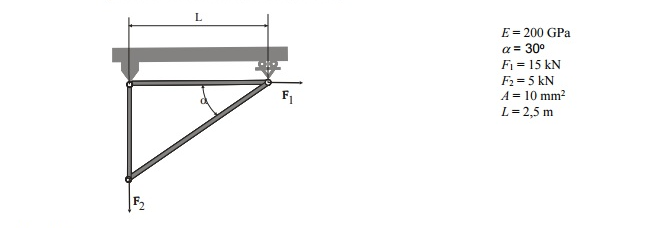
\includegraphics[scale=0.6]{pictures/chapter_fem/problem_glavas.png}
\caption{Zadatak}
\label{fig:problem__not_noted}
\end{center}
\end{figure}

Na slici vidimo problem koji moramo riješiti. Sa slike možemo očitati da se problem sastoji od 3 štapna konačna elementa spojena u 3 zajednička čvora. Također, očito je da je gornji lijevi čvor (čvor 1) fiksan, to jest on se ne može micati (ima 0 stupnjeva slobode). Gornji desni čvor (čvor 2) je slobodan samo u jednom smjeru te se može pomicati lijevo-desno, te donji čvor (čvor 3) nema nikakva ograničenja što mu daje mogućnost pomaka po cijeloj ravnini (2 stupnja slobode). \\

Za prvi dio zadatka koji je preduvjet za računanje pomaka čvorova i sile u štapovima moramo izračunati statičke sile u čvorovima i štapovima. \\
Radi lakšeg snalaženja konstruiramo vlastitu notaciju tako da je $L_2$ duljina između čvora 1 i 3, a $L_3$ duljina između čvorova 2 i 3. Na slici \ref{fig:problem_noted} su označeni i lokalni koordinatni sustavi za svaki konačni element s plavom bojom te globalni koordinatni sustav s crvenom. Također osim sila $F_1$ i $F_2$ označene su i sile $Fa_x$, $Fa_y$ i $Fb_y$.

\begin{figure}[h!t]
\begin{center}
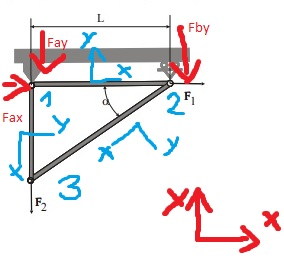
\includegraphics[scale=0.9]{pictures/chapter_fem/problem_glavas_notacija.jpg}
\caption{Slika s oznakama sila, čvorova i koordinatnih sustava}
\label{fig:problem_noted}
\end{center}
\end{figure}

Prvo izračunamo duljine preostalih štapova:
$$ L_2 = L * \tan{\alpha} = 2.5 * \tan{30} = 1.44337 m$$
$$ L_3 = \sqrt{L^2 + L^2_2} = 2.88675 m $$

Statička sila po koordinatnim osima mora biti jednaka nuli.
Statički proračun sila u štapovima i reakcija u osloncima:
$$ \sum x = 0 $$
$$ Fa_x + F_1 = 0 $$
$$ Fa_x = -F_1 = -15000 N $$
\newline

$$ \sum Mb_x = 0 $$
$$ -Fa_y * L - F_2 * L = 0 $$
$$ Fa_y = \frac{-F_2 * L}{L} = -F_2 = -5000 N $$
\newline

$$ \sum y = 0 $$
$$ -Fb_y - Fa_y - F_2 = 0 $$
$$ Fb_y = -F_2 - Fa_y = 5000 N - 5000 N = 0 N $$
\newline


Da bi mogli koristiti metodu konačnih elemenata moramo uskladiti lokalni i globalni koordinatni sustav tako da se pomaci za svaki čvor računaju u pravom smjeru. Računamo transformacijske matrice i globalne matrice krutosti za sve konačne elemente. \par

\textbf{Konačni element broj 1 (štap između čvorova 1 i 2):} \\
Os $x$ lokalnog koordinatnog sustava usmjerena je od čvora 1 prema 2 stoga se lokalni i globalni koordinatni sustavi poklapaju te je kut između globalnih i lokalnih os $0^\circ$. \\
Lokalna matrica krutosti:
\begin{equation}
    k_1 = 
    \begin{bmatrix}
    1 & 0 & -1 & 0 \\
    0 & 0 & 0 & 0 \\
    -1 & 0 & 1 & 0 \\
    0 & 0 & 0 & 0 \\
    \end{bmatrix} * \frac{E * A}{L}
\end{equation}
Transformacijska matrica:
\begin{equation}
    T_1 = I =
    \begin{bmatrix}
    1 & 0 & 0 & 0 \\
    0 & 1 & 0 & 0 \\
    0 & 0 & 1 & 0 \\
    0 & 0 & 0 & 1 \\
    \end{bmatrix} = T^{-1}
\end{equation}
Globalna matrica krutosti:
\begin{equation}
    K_1 = T^{-1}_1 * k1 * T_1 =
    \begin{bmatrix}
    800000 & 0 & -800000 & 0 \\
    0 & 0 & 0 & 0 \\
    -800000 & 0 & 800000 & 0 \\
    0 & 0 & 0 & 0 \\
    \end{bmatrix}
\end{equation}

\textbf{Konačni element broj 2 (štap između čvorova 1 i 3):} \\
Os $x$ lokalnog koordinatnog sustava usmjerena je od čvora 1 prema 3 stoga je kut između globalne i lokalne koordiantene osi $x$ jednak $270^\circ$. \\
Lokalna matrica krutosti:
\begin{equation}
    k_2 = 
    \begin{bmatrix}
    1 & 0 & -1 & 0 \\
    0 & 0 & 0 & 0 \\
    -1 & 0 & 1 & 0 \\
    0 & 0 & 0 & 0 \\
    \end{bmatrix} * \frac{E * A}{L_2}
\end{equation}
Transformacijske matrica:
\begin{equation}
    T_2 =
    \begin{bmatrix}
    0 & -1 & 0 & 0 \\
    1 & 0 & 0 & 0 \\
    0 & 0 & 0 & -1 \\
    0 & 0 & 1 & 0 \\
    \end{bmatrix}, \qquad
    T^{-1}_2 =
    \begin{bmatrix}
    0 & 1 & 0 & 0 \\
    -1 & 0 & 0 & 0 \\
    0 & 0 & 0 & 1 \\
    0 & 0 & -1 & 0 \\
    \end{bmatrix}
\end{equation}

Globalna matrica krutosti:
\begin{equation}
    K_2 = T^{-1}_2 * k2 * T_2 =
    \begin{bmatrix}
    0 & 0 & 0 & 0 \\
    0 & 1385646.0921316 & 0 & -1385646.0921316 \\
    0 & 0 & 0 & 0 \\
    0 & -1385646.0921316 & 0 & 1385646.0921316 \\
    \end{bmatrix}
\end{equation}

\textbf{Konačni element broj 2 (štap između čvorova 2 i 3):} \\
Os $x$ lokalnog koordinatnog sustava usmjerena je od čvora 2 prema 3 stoga je kut između globalne i lokalne koordiantene osi $x$, pa i $y$ jednak $210^\circ$. \\
Lokalna matrica krutosti:
\begin{equation}
    k_3 = 
    \begin{bmatrix}
    1 & 0 & -1 & 0 \\
    0 & 0 & 0 & 0 \\
    -1 & 0 & 1 & 0 \\
    0 & 0 & 0 & 0 \\
    \end{bmatrix} * \frac{E * A}{L_3}
\end{equation}
Transformacijske matrica:
\begin{equation}
    T_3 =
    \begin{bmatrix}
    -\frac{\sqrt{3}}{2} & -\frac{1}{2} & 0 & 0 \\
    \frac{1}{2} & -\frac{\sqrt{3}}{2} & 0 & 0 \\
    0 & 0 & -\frac{\sqrt{3}}{2} & -\frac{1}{2} \\
    0 & 0 & \frac{1}{2} & -\frac{\sqrt{3}}{2} \\
    \end{bmatrix}, \qquad
    T^{-1}_3 =
    \begin{bmatrix}
    -\frac{\sqrt{3}}{2} & \frac{1}{2} & 0 & 0 \\
    -\frac{1}{2} & -\frac{\sqrt{3}}{2} & 0 & 0 \\
    0 & 0 & -\frac{\sqrt{3}}{2} & \frac{1}{2} \\
    0 & 0 & -\frac{1}{2} & -\frac{\sqrt{3}}{2} \\
    \end{bmatrix}, \qquad
\end{equation}

Globalna matrica krutosti:
\begin{equation}
    K_3 = T^{-1}_3 * k3 * T_3 =
    \begin{bmatrix}
    519615 & 300000 & -519615 & -300000 \\
    300000 & 173205 & -300000 & -173205 \\
    -519615 & -300000 & 519615 & 300000 \\
    -300000 & -173205 & 300000 & 173205 \\
    \end{bmatrix}
\end{equation}

Prije zbrajanja matrica krutosti pojedinih elemenata potrebno ih je proširiti na odgovarajuće dimenzije. Time dobivamo iduće matrice za konačne elemente:

\begin{equation}
\label{eq:prosirena_k1}
    K_1 =
    \begin{bmatrix}
    800000 & 0 & -800000 & 0 & 0 & 0 \\
    0 & 0 & 0 & 0 & 0 & 0 \\
    -800000 & 0 & 800000 & 0 & 0 & 0 \\
    0 & 0 & 0 & 0 & 0 & 0 \\
    0 & 0 & 0 & 0 & 0 & 0 \\
    0 & 0 & 0 & 0 & 0 & 0 \\
    \end{bmatrix}
\end{equation}

\begin{equation}
\label{eq:prosirena_k2}
    K_2 =
    \begin{bmatrix}
    0 & 0 & 0 & 0 & 0 & 0 \\
    0 & 1385646.0921316 & 0 & 0 & 0 & -1385646.0921316 \\
    0 & 0 & 0 & 0 & 0 & 0 \\
    0 & 0 & 0 & 0 & 0 & 0 \\
    0 & 0 & 0 & 0 & 0 & 0 \\
    0 & -1385646.0921316 & 0 & 0 & 0 & 1385646.0921316 \\
    \end{bmatrix}
\end{equation}

\begin{equation}
\label{eq:prosirena_k3}
    K_3 =
    \begin{bmatrix}
    0 & 0 & 0 & 0 & 0 & 0 \\
    0 & 0 & 0 & 0 & 0 & 0 \\
    0 & 0 & 519615 & 300000 & -519615 & -300000 \\
    0 & 0 & 300000 & 173205 & -300000 & -173205 \\
    0 & 0 & -519615 & -300000 & 519615 & 300000 \\
    0 & 0 & -300000 & -173205 & 300000 & 173205 \\
    \end{bmatrix}
\end{equation}

Sada spajanjem matrica krutosti (\ref{eq:prosirena_k1}), (\ref{eq:prosirena_k2}) i (\ref{eq:prosirena_k3}) dobivamo globalnu matricu krutosti čitave strukture.

\begin{equation}
\label{eq:globalna_matrica_krutosti}
    K = K_1 + K_2 + K_3 =
    \begin{bmatrix}
    800000 & 0 & -800000 & 0 & 0 & 0 \\
    0 & 1385646.09 & 0 & 0 & 0 & -1385646.09 \\
    -800000 & 0 & 1385646.09 & 300000 & -519615 & -300000 \\
    0 & 0 & 300000 & 173205 & -300000 & -173205 \\
    0 & 0 & -519615 & -300000 & 519615 & 300000 \\
    0 & -1385646.09 & -300000 & -173205 & 300000 & 1558851.25 \\
    \end{bmatrix}
\end{equation}

U prvom dijelu zadatka izračunali smo sile, te sad možemo pomoću njih konstruirati vektor opterećenja.
\begin{equation}
\label{eq:vektor_opterecenja}
    F =
    \begin{bmatrix}
    Fa_x \\ Fa_y \\ F_1 \\ Fb_y \\ 0 \\ F_2 \\
    \end{bmatrix}
    =
    \begin{bmatrix}
    -15000 \\ -5000 \\ 15000 \\ 0 \\ 0 \\ -5000 \\
    \end{bmatrix}
\end{equation}

Sa slike \ref{fig:problem__not_noted} bili smo očitali da se pomaci mogu dogoditi samo u čvorovima 2 i 3 stoga vektor pomaka koji želimo izračunati izgleda:
\begin{equation}
\label{eq:vektor_pomaka}
    u =
    \begin{bmatrix}
    0 \\ 0 \\ u_{x2} \\ 0 \\ u_{x3} \\ u_{y3} \\
    \end{bmatrix}
\end{equation}

Sad se pomoću vektora opterećenja (\ref{eq:vektor_opterecenja}), matrice krutosti (\ref{eq:globalna_matrica_krutosti}) računa vektor pomaka (\ref{eq:vektor_pomaka}) po formuli $F = K * u $. Uklanjanjem dijelova gdje nema pomaka dobivamo idući sustav jednadžbi:
\begin{equation}
\label{eq:racunanje_pomaka}
    \begin{bmatrix}
    15000 \\ 0 \\ -5000 \\
    \end{bmatrix}
    =
    \begin{bmatrix}
    1319615.48 \\ -519615 \\ -300000 \\
    -519615 \\ 519615 \\ 300000 \\
    -300000 \\ 300000 \\ 1558851.25 \\
    \end{bmatrix}
    *    
    \begin{bmatrix}
    u_{x2} \\ u_{x3} \\ u_{y3} \\
    \end{bmatrix}
\end{equation}

Rješavanjem sustava dobivamo vektor pomaka
\begin{equation}
\label{eq:vektor_pomaka_kratki}
    u =
    \begin{bmatrix}
    0.01875 \\ 0.0208333 \\ -0.00360843 \\
    \end{bmatrix}
\end{equation}

te sada cjeloviti vektor pomaka glasi:
\begin{equation}
\label{eq:vektor_pomaka_cijeli}
    u =
    \begin{bmatrix}
    0 \\ 0 \\ 0.01875 \\ 0 \\ 0.0208333 \\ -0.00360843 \\
    \end{bmatrix}
\end{equation}

Da bi odredili reakcije oslonaca množimo cjelovitu matricu krutosti (\ref{eq:globalna_matrica_krutosti}) sa cjelovitim vektorom pomaka (\ref{eq:vektor_pomaka_cijeli}) $f = K * u$ i dobivamo
\begin{equation}
\label{eq:reakcije_oslonaca}
    f =
    \begin{bmatrix}
    -15000 \\ 
    5000 \\ 
    15000 \\ 
    4.54747 \times 10^{-13} \\ 
    -1.818989 \times 10^{-12} \\ 
    -5000 \\
    \end{bmatrix}
\end{equation}

Za određivanje unutrašnjih sila u štapovima (konačnim elementima) potrebni su nam ukupni pomaci po konačnim elemenata što zahtjeva vraćanje pomaka iz globalnog koordinatnog sustava u lokalni koji se dobiva globalnog množenjem pomaka s odgovarajućom matricom transformacije. Za konačni element 1 ukupni pomak glasi 
\begin{equation}
\label{eq:apsolutni_pomak}
\delta u_1 = u_{x2} - u_{x1}
\end{equation}
Pomak u lokalnom koordinatnom sustavu dobivamo s:
\begin{equation}
\label{eq:transformacija_u_lokalni}
    U_1 = T_1 * u_1 = I * u_1 =
    \begin{bmatrix}
    1 & 0 & 0 & 0 \\
    0 & 1 & 0 & 0 \\
    0 & 0 & 1 & 0 \\
    0 & 0 & 0 & 1 \\
    \end{bmatrix} 
    *
    \begin{bmatrix}
    0 \\ 0 \\ 0.01875 \\ 0 \\
    \end{bmatrix}
    = 
    \begin{bmatrix}
    0 \\ 0 \\ 0.01875 \\ 0 \\
    \end{bmatrix}
\end{equation}
Apsolutni pomak konačnog elementa dobivamo iz jednadžbe (\ref{eq:apsolutni_pomak}) i iznosi $$\delta u_1 = 0.01875 - 0 = 0.1875 $$
Analogno se dobivaju i apsolutni pomaci konačnih elemenata 2 i 3 koji iznose: 
$$\delta u_2 = 0.003608425$$
$$\delta u_3 = 0$$
Sada imamo sve informacije za izračunati sile u svakom štapu (konačnom elementu) koje iznose:
$$p_1 = \frac{E * A}{L} * \delta u_1 = 15000 N$$
$$p_2 = \frac{E * A}{L_2} * \delta u_2 = 5000 N$$
$$p_3 = \frac{E * A}{L_3} * \delta u_3 = 0 N $$

Ovaj primjer pokazao je na jednostavnoj strukturi što se sve treba izračunati prije dobivanja krajnjih rezultata. Rješavanje se temeljilo na metodi direktne formulacije konačnih elemenata (Direct stiffness method) o kojoj se više detalja može naći u \cite{direct_stiffness_method_article}, \cite{direct_stiffness_method} i u šestom poglavlju \cite{jurica_soric} koja je razvijena posebno za učinkovito i lako implementiranje u računalni softver za procjenu kompliciranih struktura koje sadrže veliki broj jednostavnih konačnih elemenata. Također, danas se velik broj program za rješavanje metode konačnih elemenata temelji na upravo toj metodi.



\chapter{OOFEM}	
OOFEM je objektno orijentirani program otvorenoga koda (open source) dizajniran za rješavanje mehaničkih, transportnih i fluidnih problema pomoću konačnih elemenata koji radi na različitim platformama \cite{oofem-web}. U ovom poglavlju detaljno opisujemo softverski program OOFEM. U početku dajemo kratak opis kako se je program razvijao, te njegovo trenutno stanje. U drugom dijelu dajemo opis strukture koda te arhitektonske odluke. Zatim slijede dijelovi gdje se opisuju postojeći konačni elementi i materijali za te konačne elemente te kako dodati nove. Nakon što završimo opis samog programa slijedi što OOFEM očekuje kao ulazne podatke i mogućnosti što sve OOFEM može izračunati. Kako je za OOFEM predviđeno da čita ulazne podatke iz datoteke autori su radi trenutnog stanja u praksi gdje programski jezik Python dobiva sve više na važnosti i popularnosti odlučili omogućiti zadavanje ulaznih podataka programski putem Python-a. U dijelu \ref{poglavlje:koristenje_pythona} objašnjavamo što sve i kako možemo koristiti Python pri zadavanju ulaznih podataka. U posljednjem dijelu poglavlja prikazujemo kako analizirati dobivene rezultate što uključuje validaciju vrijednosti i naknadnu analizu putem vizualizacijskih alata radi lakšeg snalaženja u moru vrijednosti sila i naprezanja. Ovo poglavlje temelji se na web stranici i dokumentaciji OOFEM-a. \cite{oofem_article} \cite{oofem-web}

\section{O OOFEM-u}
Cilj OOFEM-a je razviti djelotvoran i robustan alat za izračune metode konačnih elemenata te osigurati modularno i proširivo okruženje za budući razvoj. OOFEM je izdan pod licencom za slobodan softver, GNU Lesser General Public License (LGPL). Više o tipu licence može se pronaći na \cite{gnu_licence}, ali ukratko ova licenca dopušta slobodno korištenje, modifikaciju i redistribuciju softvera. OOFEM je u kontinuiranom razvoju od 1997. godine. Projekt je započeo 1993. godine kao dio doktorske disertacije Boreka Patzaka o računalnom modeliranju betonskih konstrukcija i financiran je djelomično od strane ministarstva znanosti i znanstven zaklade Češke Republike, fondova Europske unije i industrije (LMAT, www.lmat-uk.com). Prema Github-u \cite{oofem_github}  i Openhub-u \cite{oofem_openhub} projekt sadrži nešto manje od 300,000 linija koda i na njemu su radila 42 suradnika. Openhub procjenjuje da je u taj projekt uloženo 76 godina rada (COCOMO model) što ga s prosječnom cijenom rada stručne osobe od 200,000 kn po godini čini projekt vrijedan 15,200,000 kuna. Važno je još napomenuti da je većina koda napisana u C++-u koji čini 94\% projekta i da je projekt dobro dokumentiran (28\%, što ga stavlja iznad prosjeka). OOFEM ima mnogo značajki, od kojih nama najvažnije su iduće:
\begin{itemize}
    \item Objektno orijentirana arhitektura
    \item Modularna i proširiva jezgra za računanje metode konačnih elemenata (OOFEMlib)
    \begin{itemize}
        \item potpuno proširiva - jezgra programa se može proširiti u bilo kojem "smjeru". Moguće je dodavanje nove vrste konačnih elementa, novog modela materijala s bilo kojim tipom i brojem internih parametara povijesti, novim graničnim uvjetima, numeričkim algoritmima ili modulima analize, kao i sposobnošću dodavanja i upravljanja proizvoljnim stupnjevima slobode.
        \item neovisna formulacija problema, numeričkog rješavanja i pohrane podataka - jezgra pruža neovisne apstrakcije za analizu, opću numeričku metodu i pohranu podataka (rijetke "sparse" matrice). Koncept mapiranja komponenata omogućuje samostalno formuliranje problema i numeričke metode i omogućuje korištenje bilo koje prikladne numeričke metode za rješavanje problema bez promjene. Ovaj koncept dodatno je poboljšan apstraktnim sučeljem za rijetke matrice, koje omogućuje samostalno formuliranje numeričke metode nad rijetkim matricama.
        \item potpuna podrška za ponovno pokretanje - jezgra podržava potpuno ponovno pokretanje iz bilo kojeg prethodno spremljenog stanja.
        \item stupnjevita analiza - omogućuje grupiranje osnovnih problema, prijenos i dijeljenje rješenja polja između osnovnih potproblemima. Opći dizajn omogućuje korištenje različitih diskretizacija za osnovne podprobleme.
        \item paralelna podrška za procesiranje - temeljena na rastavljanju domene, paradigmama slanja poruka i dinamičnom balansiranju opterećenja računanja. Mnoge strukturne analize mogu se izvoditi paralelno čime se dobivaju velika ubrzanja.
        \item efikasni algoritmi za rješavanje rijetkih matrica - dostupni su izravni i iterativni algoritmi. Metode izravnog rješavanja uključuju simetrično i nesimetrično rješavanje. Iterativne metode podržavaju mnoge rijetke oblike pohrane i dolaze s nekoliko pretpostavki. Dostupna su i sučelja za biblioteke linearnih metoda za programe poput IML, PETSc (serijski i paralelni), PARDISO, SuperLu i SPOOLES.
        \item podrška za proširenu metodu konačnih elemenata (eXtended Finite Element Method XFEM) - ugrađena reprezentacija za globalne funkcije obogaćivanja i njihov geometrijski opis. Generalna integracijska pravila pružaju podršku za implementiranje XFEM baziranih algoritama.
    \end{itemize}
    \item Modula za strukturnu mehaniku
        \begin{itemize}
            \item različite procedure za analizu - linearna statička i linearnu dinamička (analiza vrijednosti svojstvenih vektora, direktne metode integracije - implicitno i eksplicitno); nelinearna statička (CALM rješavanje), nelinearna dinamička (eksplicitna, paralelna verzija)
            \item velika biblioteka materijala, uključujući najsuvremenije modele za nelinearne mehanike prijeloma kvazi lomljivih materijala. Više o tome u \ref{poglavlje:materials_in_oofem}.
            \item prilagodiva analiza - linearna i nelinearna 
            \item napredne značajke modeliranja - čvorovi robovi, lokalni koordinatni sustavi, aktivacija / deaktivacija elemenata i još mnogo toga.
            \item paralelna analiza - eksplicitna nelinearna dinamika koja koristi metodu razlaganja domene, linearna i nelinearna statička (zahtijeva PETSC).
        \end{itemize}
    \item Naknadna analiza (post processing)
        \begin{itemize}
            \item ugrađeno X-window procesiranje
            \item pretvorba izlaza u VTK format za korištenje vizualizacijskih alata poput MayaVi ili ParaView za vizualizaciju na različitim platformama
        \end{itemize}
    \item Sučelje prema generatorima mreža T3d i Targe2, te alat za unos podataka iz UNV formata
    \item Sučelje prema bibliotekama za dobivanje svojstvenih vrijednosti (trenutno su podržani PETSc, SLEPc, IML, PARDISo, SuperLu i SPOOLES) 
\end{itemize}
Osim već nabrojanih OOFEM ima i module za rješavanje problema dinamike fluida i prijenosa topline.

\section{Struktura koda OOFEM-a}
\label{poglavlje:struktura_koda}
U poglavlju o metodi konačnih elemenata vidjeli smo da postoji više načina rješavanja i nekoliko različitih problema (strukturna analiza, analizi fluida, prijenosu topline, elektrostatičkim problemi) koji se rješavaju na gotovo isti način, kao i velik broj različitih konačnih elemenata koji moraju poštivati zajednička svojstva. Sve to nam nameće ideju o objektno orijentiranom pristupu. Tim su se principom vodili i arhitekti OOFEM programa. Tako se cijela arhitektura OOFEM-a bazira na nasljeđivanju općenitih apstraktnih klasa koje implementiraju specifična svojstva za određeni problem. Na slici \ref{fig:numerical_method_inheritance} vidimo jedan takav primjer.
\begin{figure}[h!t]
\begin{center}
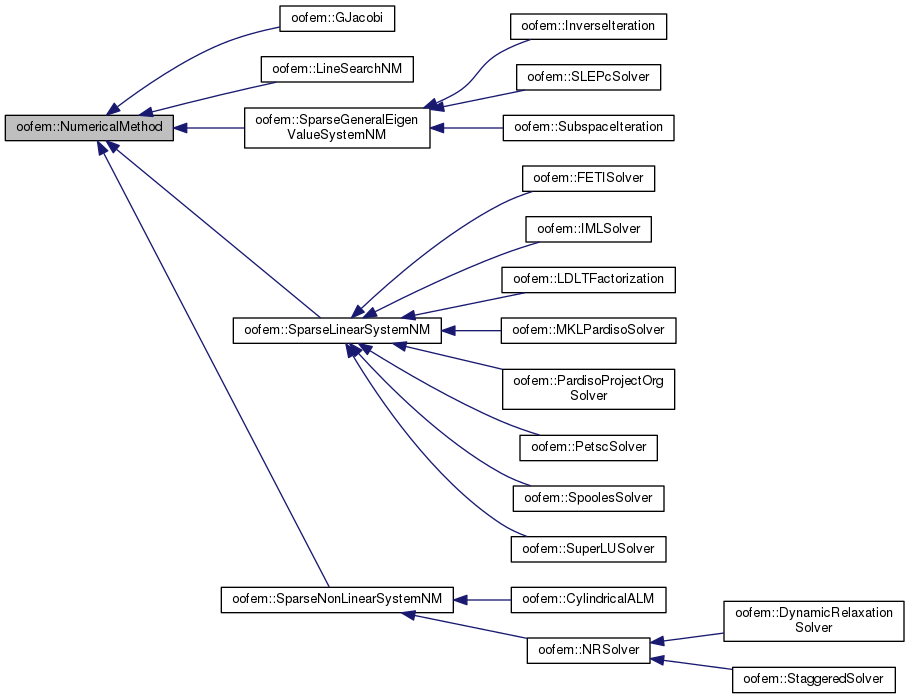
\includegraphics[scale=0.46]{pictures/chapter_oofem/NumericalMethod_inheritance.png}
\caption{Dijagram nasljeđivanja apstraktne klase NumericalMethod \cite{oofem_reference}}
\label{fig:numerical_method_inheritance}
\end{center}
\end{figure}
Na slici je prikazan dijagram nasljeđivanja za osnovnu klasu koja opisuje što sve numeričke metode za specifične probleme poput rješavanja linearnog sustava moraju implementirati. Također na slici vidimo da nasljeđivanje ide u dubinu do čak 3 razine čemu je razlog to što se na prvoj razini grana na numeričke metode koje rješavaju različite probleme, a tek kasnije uvode implementacije za rješavanje tih problema. \par
Nadalje, dat ćemo opis svih najvažnijih klasa u OOFEM-u, njihove uloge, međusobnu komunikaciju i stabla nasljeđivanja. Informacije su dobivene iz izvornog koda na \cite{oofem_github} i automatsko kreiranoj dokumentaciji  na \cite{oofem_reference} i \cite{oofem_programmer}. Okosnica program su iduće klase: EngngModel, Domain, NumericalMethod i FEMComponent. Iz tih klasa izniču gotovo sve ostale funkcionalnosti te su upravo one zaslužne za apstrakciju i objektno orijentirani pristup. \par

Klasa koja obuhvaća, te kasnije i inicijalizira sve ostale je \textbf{EngngModel}. EngngModel je apstrakcija za problem koji se razmatra. Ona je prva klasa koji se inicijalizira i predstavlja vrstu analize koju treba izvršiti, te implementira komunikaciju sa svim svojim atributima. Izvedene klase poput FluidModel i LinearStatic "znaju" sastaviti jednadžbe i fizičko značenje pojedinih komponenti. One su odgovorne za formiranje upravljačke jednadžbe za svaki korak rješavanja, obično zbrajanjem doprinosa pojedinih elemenata i čvorova. Glavne funkcije klase EngngModel su:
\begin{itemize}
    \item Parsiranje ulaza (ulazne datoteke) na zasebne domene i spremanje rezultata
    \item Spremanje i vraćanje stanja u/iz kontekstnih datoteka
    \item Sastavljanje jednadžbi zbrajanjem doprinosa iz problemskih domena (obično od čvorova i elemenata)
    \item Rješavanje problema opisanih jednadžbama pomoću prikladnih numeričkih metoda. To zahtijeva povezivanje numeričkih metoda karakterističnih elemenata s komponentama jednadžbi. EngngModel mora mapirati svaku komponentu jednadžbe (koja ima fizičko značenje) odgovarajućoj numeričkoj komponenti numeričke metode
    \item Prekinuti vremenski korak ažuriranjem vrijednosti čvorova i elementa (uključujući ažuriranje integracijskih točaka)
\end{itemize}
Koje sve probleme OOFEM "zna" riješiti možemo vidjeti tako da pogledamo tko sve implementira klasu EngngModel. Grafički prikaza toga dan je na slici \ref{fig:engngModel_inheritance}

\begin{figure}[h!t]
\begin{center}
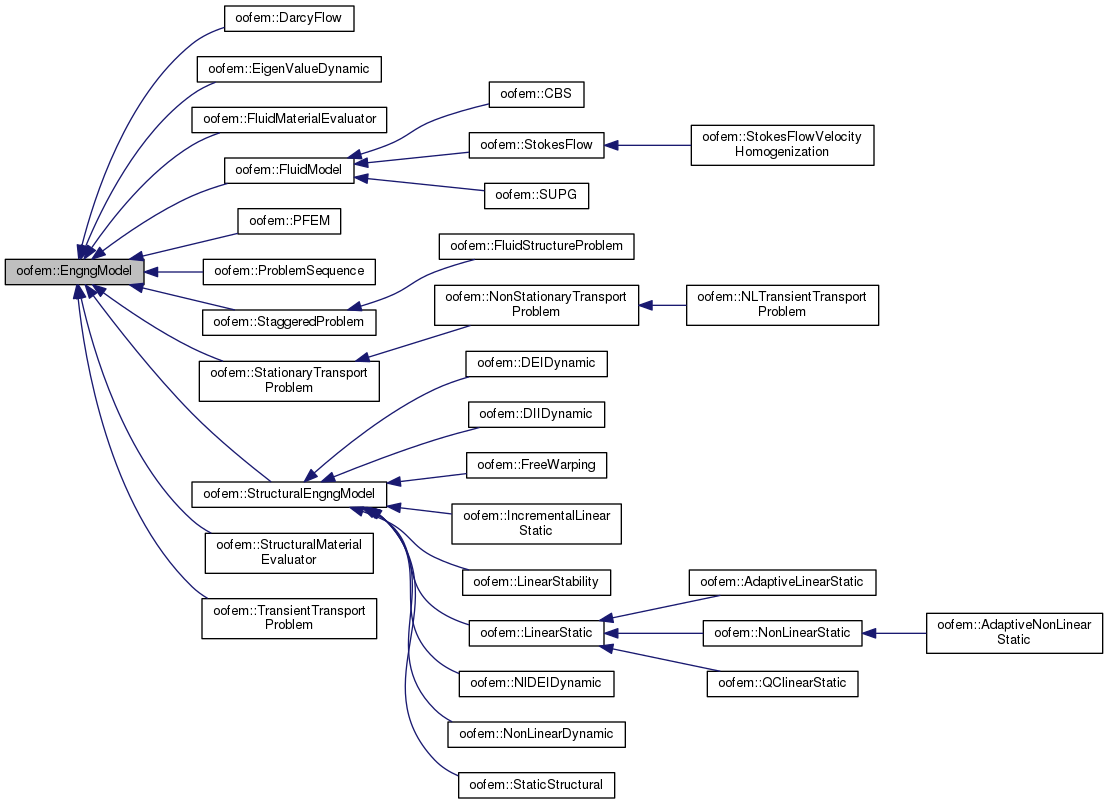
\includegraphics[scale=0.38]{pictures/chapter_oofem/EngngModel_inheritance.png}
\caption{Dijagram nasljeđivanja apstraktne klase EngngModel \cite{oofem_reference}}
\label{fig:engngModel_inheritance}
\end{center}
\end{figure}

\par
Iduća važna klasa koja je sadržana kao atribut unutar EngngModel klase je \textbf{Domain}. Mreža čvorova i elemenata je reprezentirana pomoću nje, te su unutar Domain klase spremljene sve komponente modela metode konačnih elemenata poput čvorova, stupnjeva slobode (Degree Of Freedom, DOF), materijala, rubnih uvjeta itd. Svaki EngngModel ima barem jednu domenu koja omogućuje apstrakciju te se brine za daljnju komunikaciju s njezinim elementima. Najvažnije funkcije domene su:
\begin{itemize}
    \label{text:domain}
    \item Konstruiranje objekata pročitanih s ulaza. To uključuje čitanje i parsiranje mreže s ulaza te konstrukciju odgovarajućih komponenata pravoga tipa.
    \item Pružanje generaliziranog pristupa pojedinim komponentama domene.
    \item Filtriranje izlaza za određene korake, elemente i čvorove tokom rješavanja
\end{itemize}

\par

Kao što smo već vidjeli na slici \ref{fig:numerical_method_inheritance} apstraktna klasa koja omogućava lagano dodavanje novih matematičkih metoda rješavanja pojedinih problema je \textbf{NumericalMethod}. Engng model može koristiti različite numeričke metode, ovisno, na primjer, o veličini problema ili prethodnoj konvergenciji. Svaka pojedina instanca Engng modela odgovorna je za mapiranje njezinih jednadžbi na odgovarajuće numeričke komponente. Takvo mapiranje omogućuje implementiranje numeričkih metoda neovisno od određenog fizičkog problema. Samim time, numerička metoda može predstavljati i sučelje za algoritam napisan u C-u ili Fortranu. Klase izvedene iz numeričke metode trebale bi objaviti sučelje za specifičnu vrstu problema (poput rješenja linearnog sustava). Treba naglasiti da sve numeričke metode koje rješavaju isti problem koriste isto sučelje (isto mapiranje) - to se provodi korištenjem iste osnovne klase osnovnih problema. Primjer toga je problem rješavanja rijetkog linearnog sustava deklariranog klasom SparseLinearSystemNM. Stoga je moguće riješiti problem s bilo kojom prikladnom numeričkom metodom za klasifikaciju i ostaviti cijeli model, uključujući i mapiranje, nepromijenjen jer sve instance klase pružaju zajedničko sučelje. \par

Klasa s najvećim brojem nasljeđivanja i najdubljim stablom je \textbf{FEMComponent} klasa. Na slici \ref{fig:FEMComponent_inheritance} se može vidjeti to stablo koja radi svoje veličine nije moglo stati stoga nekim čvorovima nisu ni sva djeca prikazana.

\begin{figure}[h!t]
\begin{center}
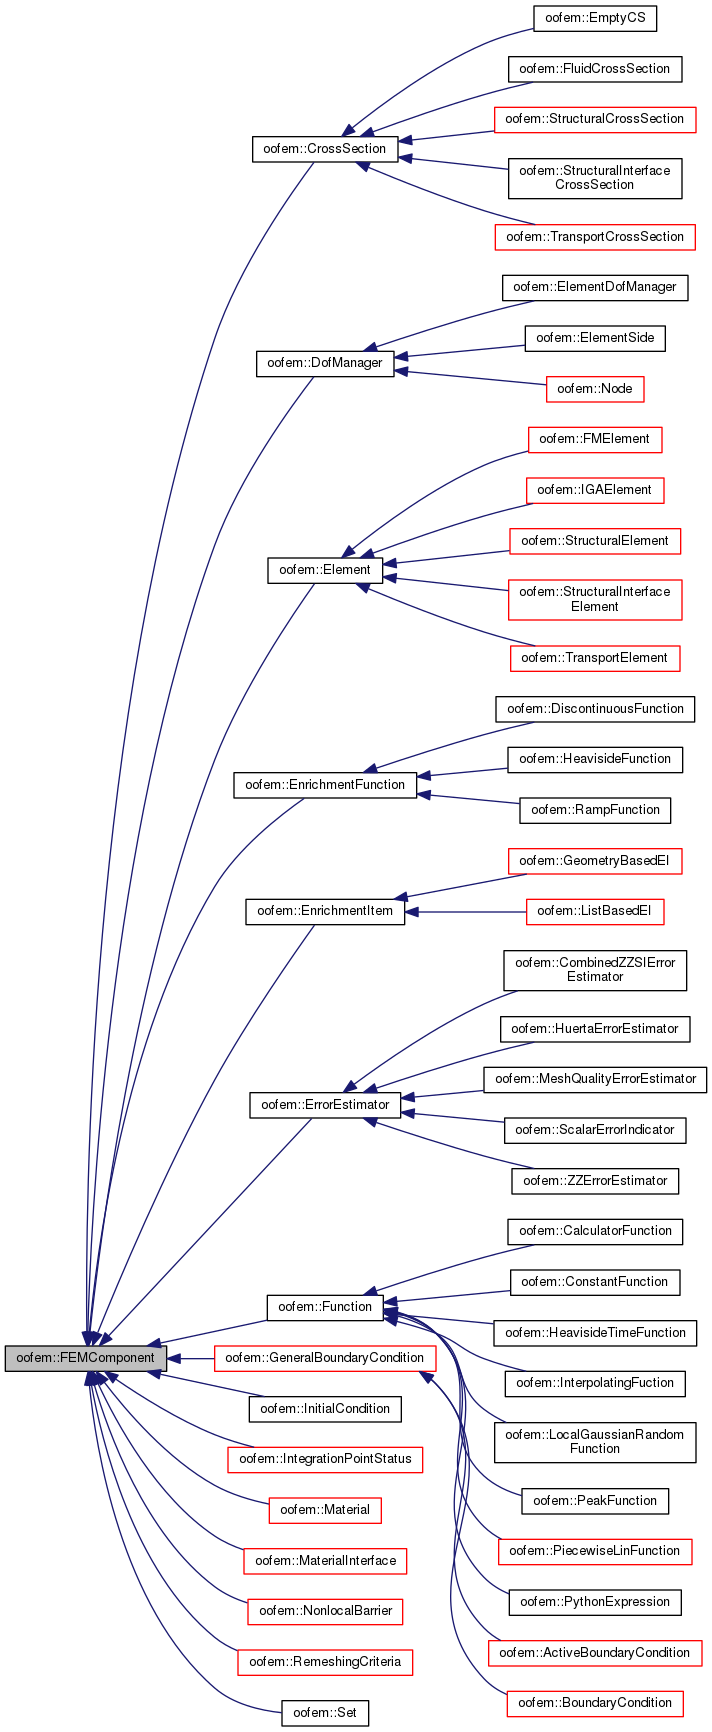
\includegraphics[scale=0.26]{pictures/chapter_oofem/FEMComponent_inheritance.png}
\caption{Dijagram nasljeđivanja apstraktne klase FEMComponent. Čvorovima s crvenim okvirom nisu prikazana djeca. \cite{oofem_reference}}
\label{fig:FEMComponent_inheritance}
\end{center}
\end{figure}

FEMComponent klasu implementiraju svi objekti koji su u vezi s konačnom metodom elemenata. Tako se među klasama koje implementiraju mogu pronaći rubni uvjeti, inicijalni uvjeti, funkcije sa silama, materijali konačnih elemenata te i sami konačni elementi. FEMComponent definira atribute i metode zajedničke svim komponentama mreže: elementima, čvorovima, vremenskim koracima, materijalima, opterećenjima i funkcijama učitavanja. Ova klasa definira dva atributa zajednička svim komponentama konačnih elemenata. "Broj" koji se prvenstveno koristi za čitanje podataka u podatkovnoj datoteci i "domena" koja se koristi za komunikaciju s drugim komponentama (npr. za element koji će dobiti svoj materijal), za pristup koordinatnom sustavu i podatkovnoj datoteci. U idućim potpoglavljima detaljnije ćemo opisati klase koje opisuju materijale od kojih se konačni elementi mogu sastojati i klase konačnih elemenata. \par

Zanimljivo je još i vidjeti kako sve te klase međusobno komuniciraju, to jest kako su one povezane. Dobar uvid u to nam daje slika \ref{fig:EngngModel_connections} gdje su prikazane poveznice između klasa. Na slici se vidi kako na apstraktnoj razini klase međusobno komuniciraju, to jest kako čitav softver zapravo i radi. Što se raspodijele koda u direktorije tiče, u repozitoriju \cite{oofem_github} se nalaze mnogi direktoriji od kojih ćemo se mi koncentrirati u većoj ili manjoj mjeri na iduće: bindings, doc, src i tools. U direktoriju doc se nalazi se dokumentacija u TeX obliku koja se automatski nadopunjuje iz komentara unutar koda. Generirana dokumentacija se nalazi i na \cite{oofem-web} te je bitan izvor svih informacija. Više o direktoriju bindings bit će rečeno u potpoglavlju \ref{poglavlje:koristenje_pythona} jer se tu nalazi sve potrebno za korištenje OOFEM softvera pomoću Python-a. Direktorij tools sadrži različite alate za modifikaciju ulaznih i izlaznih podataka. Posljednji i najvažniji direktoriji je src koji sadrži sam kod softvera. Unutar tog direktorija nama najvažniji bit će sm koji se odnosi na strukturnu analizu. Unutar njega nalaze se svi potrebni i nama zanimljivi elementi poput materijala, konačnih elemenata i modela rješavanja.

\begin{figure}[h!t]
\begin{center}
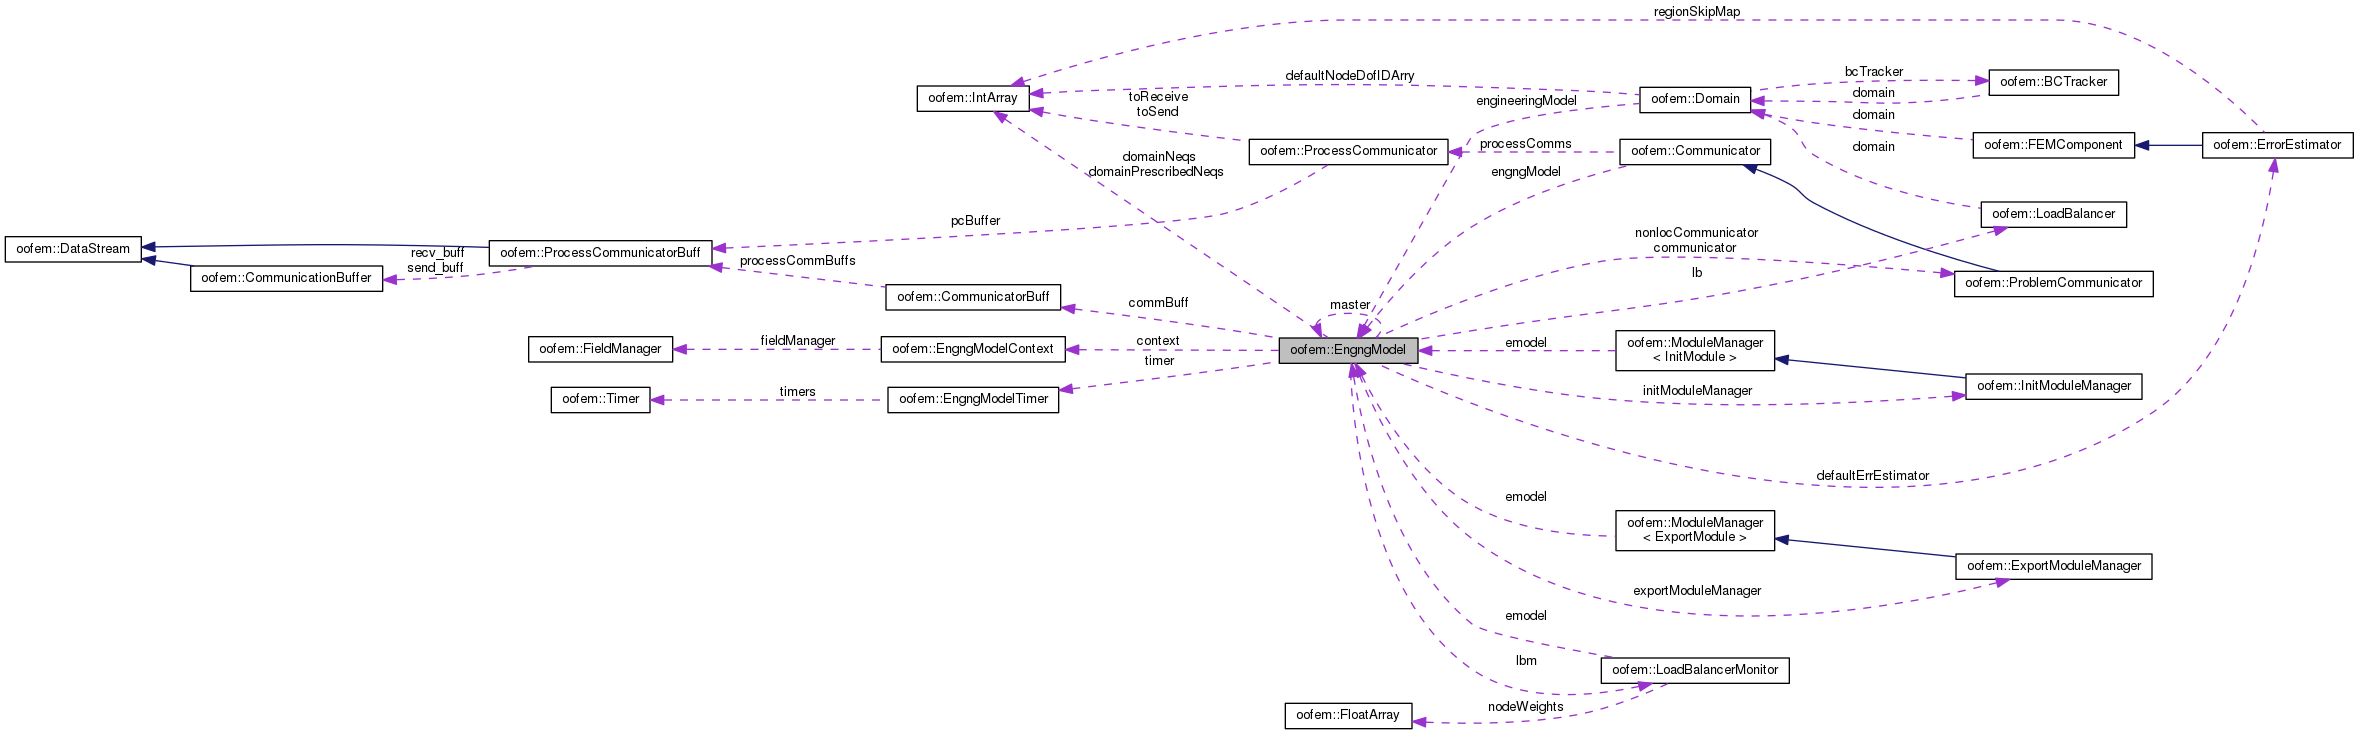
\includegraphics[scale=0.2, angle=90]{pictures/chapter_oofem/EngngModel_connections.png}
\caption{Dijagram s poveznicama između apstraktnih klasa OOFEM-a. \cite{oofem_reference}}
\label{fig:EngngModel_connections}
\end{center}
\end{figure}

\section{Materijali u OOFEM-u}
\label{poglavlje:materials_in_oofem}
Osnovna klasa za sve materijalne modele je klasa Material, izvedena iz FEMComponent. Klasa Material implementira sučelje nezavisno uz samu analizu. Dio sučelja potreban za analizu trebaju dodati izvedene klase, koje predstavljaju osnovne klase za određeni problem. Tipičan primjer je klasa \textbf{StructuralMaterial} za strukturalni materijal koji izlaže sve usluge potrebne za strukturnu analizu i na koju ćemo se kao što je rečeno u prethodnom dijelu najviše koncentrirati. Izravno izvedene klase poput SturucturalMaterial moraju implementirati specifične dijelove konačnih elemenata i poprečnog presjeka za domensku problematiku što su na primjeru klase StructuralMaterial klase StructuralElement i StructuralCrossSection koje su apstraktne osnovne klase za sve "strukturalne" konačne elemente.
Kako bi se pohranile sve potrebne varijable povijesti modela materijala, usvaja se takozvani koncept stanja. Stanje materijala može se smatrati spremnikom svih potrebnih povijesnih varijabli. Obično se pohranjuju dvije vrste varijabli, privremene i trajne. Privremene se odnose na stvarno stanje integracijske točke, ali ne moraju odgovarati globalnoj ravnoteži. Te se promjene mijenjaju tijekom iteracija pretraživanja ravnoteže. Trajne varijable odnose se na prethodno konvergirano stanje. Za svaki model materijala mora biti definiran odgovarajuće stanje i mora biti stvorena i pridružena jedinstvena instanca za svaku integracijsku točku. Za prije navedeni materijal SturcturalMaterial to je klasa StructuralMaterialStatus koja je također apstraktna te predstavlja osnovnu za implementaciju stanja pojedinih materijala. U idućem dijelu dajemo detaljan opis jednog materijala za strukturnu analizu te što je sve potrebno za njegovu implementaciju.

\subsection{Primjer materijala}
U ovom odjeljku opisat će se implementacija materijala izotropnog oštećenja. Za pokrivanje raznih modela temeljenih na izotropnom konceptu oštećenja, najprije se definira osnovna klasa IsotropicDamageMaterial koja implementira sve zajedničke značajke. Izvedene klase onda samo implementiraju određene zakone o evoluciji oštećenja.
Modeli izotropnih oštećenja temelje se na pojednostavljenoj pretpostavci da je degradacija krutosti izotropna, to jest moduli krutosti koji odgovaraju različitim smjerovima smanjuju se proporcionalno i neovisno o smjeru djelovanja sila. Posljedično, matrica krutosti oštećenja izražava se kao:
$$ D = (1 - \omega) * D_\epsilon$$
gdje je $D_\epsilon$ elastična matrica krutosti neoštećenog materijala i $\omega$ je parametar oštećenja. U početku, $\omega$ je postavljen na nulu, što predstavlja "novi" neoštećeni materijal i reagira linearno elastično. Budući da materijal prolazi kroz deformaciju širenje mikro nedostataka smanjuje krutost, što je predstavljeno rastom parametra $\omega$ oštećenja. Za $\omega = 1$, krutost u potpunosti nestaje. U trenutnom kontekstu, matrica $D$ predstavlja krutost koja se odnosi na omjer naprezanja i sile
$$\sigma = D \epsilon = (1 - \omega) D_\epsilon \epsilon$$
Slično teoriji plastičnosti, uvodi se funkcija sile $f$. U teoriji oštećenja prirodno je raditi u prostoru naprezanja i stoga funkcija sile ovisi o naprezanju i o dodatnom parametru $\kappa$, opisujući evoluciju štete. Fizikalno, $\kappa$ je skalar najveće razine napetosti koju je materijal dosegao. Funkcija sile obično ima oblik 
$$f(\epsilon, \kappa) = \widetilde{\epsilon} (\epsilon) - \kappa$$
gdje je $\widetilde{\epsilon}$ jednak naprezanju. Ostaje povezati varijablu $\kappa$ s parametrom $\omega$ oštećenjem. Budući da oba $\kappa$ i $\omega$ rastu monotonno, prikladno je pretpostaviti eksplicitnu jednadžbu:
$$ \omega = g(\kappa) $$
Važna prednost ove eksplicitne formulacije je da se sila koja odgovara danom naprezanju može izravno procijeniti, bez potrebe za rješavanjem nelinearnog sustava jednadžbi.
Ovaj opći okvir za računanje naprezanja i matrice krutosti je uobičajen za sve materijalne modele ove vrste. Dakle, prirodno je uvesti osnovnu klasu za sve modele izotropnih oštećenja koji osiguravaju opću
implementacija algoritama za evaluaciju matrice sila i krutosti. Pojedini modeli zatim pružaju samo njihov ekvivalent naprezanju i oštećenju. Tako se na primjer za definiciju naprezanja po Mazarsu (1984) dovoljno uvrstiti njegovu formulu naprezanja
$$ \widetilde{\epsilon} = \sqrt{\sum^3_{I=1} \langle \epsilon_I \rangle^2 }$$
Također, kao što je prije i navedeno za svaki materijal potrebno je implementirati i klasu stanja pa se tako implementira i IsotropicDamageMaterialStatus. Za izotropsko bazirane modele oštećenja jedina varijabla koju je potrebno pamtiti jest najveće dostignuto naprezanje ($\kappa$). Osim toga implementira se i metoda za pristupanje i promjenu naprezanja.

\begin{figure}[h!t]
\begin{center}
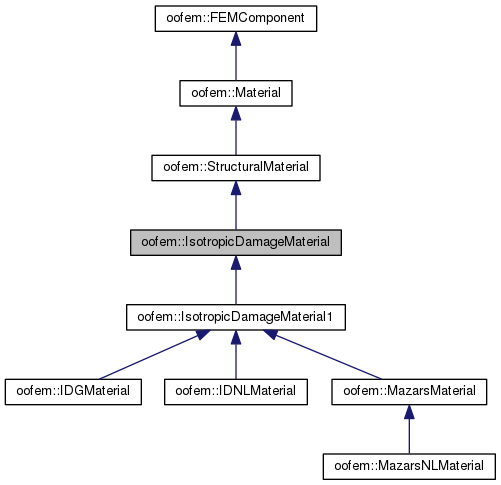
\includegraphics[scale=0.4]{pictures/chapter_oofem/IsotropicDamageMaterial_inheritance.png}
\caption{Dijagram apstraktne klase nasljeđivanja materijala izotropskog oštećenja. \cite{oofem_reference}}
\label{fig:IsotropicDamageMaterial_inheritance}
\end{center}
\end{figure}


\section{Konačni elementi u OOFEM-u}
\label{poglavlje:finite_elements_in_oofem}
Glavna bazna apstraktna klasa za sve konačne elemente je \textbf{Element}. Glavna svrha ove klase jest implementacija osnovnih značajki koje su zajedničke svim konačnim elementima (kao što su pohranjivanje referenci na materijal elementa, čvorovi, opterećenja, sastavljanje polja lokacije, pohranjivanje iz/u kontekstnu datoteku i slično). Klasa Element ne implementira niti jednu metodu koja se odnosi na određenu analizu već ih samo deklarira te dopušta izvedenim klasama da ih implementiraju. Direktna djeca obično definiraju opće usluge potrebne za određenu svrhu analize poput matrica krutosti i mase za strukturalnu analizu ili matrice procjene kapaciteta i provodljivosti za analizu prijenosa topline. Na slici \ref{fig:Element_inheritance} vidimo kako izgleda stablo nasljeđivanja klase Element. Nadalje, kao i ranije koncentrirat ćemo se na strukturalnu analizu, to jest konačne elemente koji nasljeđuju klasu \textbf{StructuralElement} koja je osnovna klasa za sve konačne elemente strukturalne analize. Konkretnije, nakon opisa klase StructuralElement opisat ćemo i klasu Truss1d koja opisuje štapni element u dvodimenizionalnom prostoru. \par


\begin{figure}[h!t]
\begin{center}
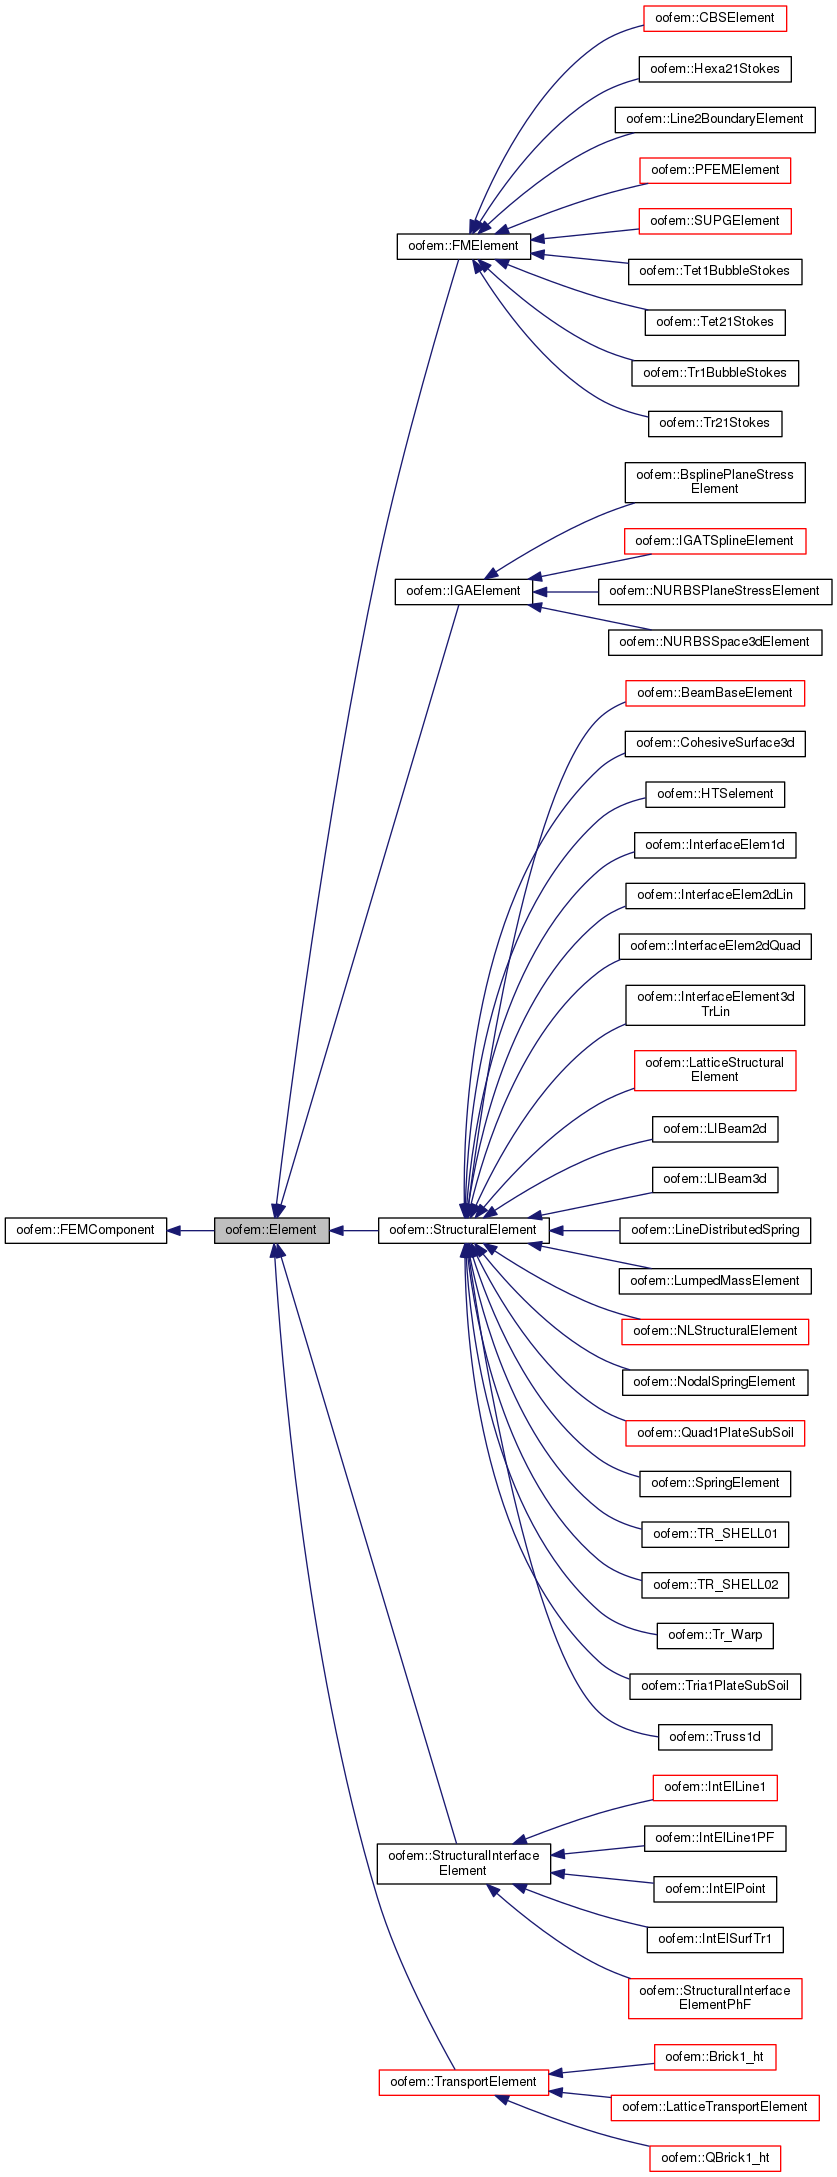
\includegraphics[scale=0.21]{pictures/chapter_oofem/Element_inhereitnace.png}
\caption{Dijagram nasljeđivanja osnovne klase Element. \cite{oofem_reference}}
\label{fig:Element_inheritance}
\end{center}
\end{figure}

Klasa StrukturalElement deklarira sve potrebne potrebne metode i atribute koje zahtijeva strukturalna analiza poput metode računanja matrica krutosti, opterećenja, naprezanja i vektora sila. 
Osnovni zadaci strukturalnog elementa su izračunavanje doprinosa globalnim jednadžbama ravnoteže (matrice mase i krutosti, različitih vektora opterećenja zbog graničnih uvjeta, sile opterećenja, toplinskog opterećenja itd.) i izračunavanje odgovarajućih naprezanja i sila iz pomaka čvorova. Radi toga se deklariraju odgovarajuće virtualne metode za računanje tih doprinosa. Ti standardni doprinosi mogu se izračunati numeričkom integracijom odgovarajućih struktura, koji tipično ovise o interpolaciji elemenata ili tipu materijala, u odnosu na volumena elemenata. Stoga je moguće osigurati opće definicije tih metoda, pod uvjetom da se primjenjuju odgovarajuće metode za računanje interpolacije materijala i da su inicijalizirana odgovarajuća integracijska pravila i uvjeti. Kao primjer toga dajemo računanje matrice krutosti. Budući da matrica krutosti elemenata doprinosi globalnoj ravnoteži, krutost će biti zatražena korištenjem metode \textit{giveCharacteristicMatrix}. Implementacija metode strukturalnog elementa uzima u obzir samo materijalnu nelinearnost (geometrijska nelinearnost se ne uzima u obzir te se za elemente u kojima geometrijska nelinearnost igra ulogu očekuje da se ova metoda nadjača). Matrica krutosti elementa može se izračunati koristeći se formulom:
$$ K = \int_V B^T D B dV $$
gdje je $B$ takozvana geometrijska matrica koja sadrži derivacije funkcija oblika, a $D$ je matrica krutosti materijala. Numerička integracija koristi se za procjenu tog integralnog. Za numeričku integraciju koristi se klasa \textit{IntegrationRule}. Pravila integracije za određeni element kreiraju se tijekom inicijalizacije elementa i pohranjuju se u polju \textit{integrationRulesArray} kao atribut klase, naslijeđen iz klase Element. \par

Nadalje slijede neki implementacijiski detalji klase \textit{Truss1d}. Nju uzimamo kao primjer što je sve potrebno implementirati za jedan konačan element ukoliko želimo dodati novi koji još nije implementiran. Također, vjerojatnost potrebe za dodavanjem novih dosta je mala jer OOFEM već sadrži oko 70tak različitih konačnih elemenata. \textit{Truss1d} (štapni element u 1D) predstavlja linearni izoparametrski rešetkasti element u 1D određen s dva čvora. Pretpostavlja se da se elementi nalaze duž x-osi. Element zahtjeva da mu je područje poprečnog presjeka određeno. Sama implementacija izvedena je u 400tinjak linija koda, a mi ćemo dati kratki opis datoteke zaglavlja i najvažnije metode koje zaglavlje deklarira kao i neke od implementacije jednostavnijih metoda. \textit{Truss1d} (štapni element) služi pri strukturalnoj analizi stoga nasljeđuje klasu \textit{StructuralElement}. Od važnijih metoda implementira virtualnu metodu computenumberOfDofs koja vraća broj 2, a označava broj stupnjeva slobode. Zatim slijede implementacija za računanje interpolacijske i geometrijske matrica. Obje metode računaju rješenja na danim integracijskim točkama koje dobivaju kao parametre. Dajemo kod za računanje interpolacijeske matrice pomaka:

\begin{lstlisting}[caption={Računanje interpolacijske matrice za štapni element u 1D}]
void
Truss1d :: computeNmatrixAt(const FloatArray &iLocCoord, FloatMatrix &answer)
// Returns the displacement interpolation matrix {N} of the receiver,
// evaluated at gp.
{
    FloatArray n;
    this->interp.evalN( n, iLocCoord, FEIElementGeometryWrapper(this) );
    // Reshape
    answer.resize(1, 2);
    answer.at(1, 1) = n.at(1);
    answer.at(1, 2) = n.at(2);
}
\end{lstlisting}

Samo zaglavlje elementa izgleda ovako:
\begin{lstlisting}[caption={Datoteka zaglavlja za štapni element u 1D}]
#ifndef truss1d_h
#define truss1d_h

...

namespace oofem {
class FEI1dLin;

/**
 * This class implements a two-node truss bar element for one-dimensional
 * analysis.
 */
class Truss1d : public StructuralElement{

...

public:
    Truss1d(int n, Domain * d);
    virtual ~Truss1d() { }

    virtual FEInterpolation *giveInterpolation() const;

    virtual void computeLumpedMassMatrix(FloatMatrix &answer, TimeStep *tStep);
    virtual void computeMassMatrix(FloatMatrix &answer, TimeStep *tStep)
    { computeLumpedMassMatrix(answer, tStep); }

    virtual int computeNumberOfDofs() { return 2; }
    virtual void giveDofManDofIDMask(int inode, IntArray &) const;

    // characteristic length (for crack band approach)
    virtual double giveCharacteristicLength(const FloatArray &normalToCrackPlane)
    { return this->computeLength(); }

    virtual double computeVolumeAround(GaussPoint *gp);
    
    virtual void computeStressVector(FloatArray &answer, const FloatArray &strain, GaussPoint *gp, TimeStep *tStep);
    virtual void computeConstitutiveMatrixAt(FloatMatrix &answer, MatResponseMode rMode, GaussPoint *gp, TimeStep *tStep);

    virtual int testElementExtension(ElementExtension ext) { return 0; }

    virtual Interface *giveInterface(InterfaceType it);

    virtual MaterialMode giveMaterialMode() { return _1dMat; }
    
    ...
    
protected:
    virtual void computeBmatrixAt(GaussPoint *gp, FloatMatrix &answer, int = 1, int = ALL_STRAINS);
    virtual void computeBHmatrixAt(GaussPoint *gp, FloatMatrix &answer);
    virtual void computeNmatrixAt(const FloatArray &iLocCoord, FloatMatrix &answer);
    virtual void computeGaussPoints();

};
} // end namespace oofem
#endif // truss1d_h

\end{lstlisting}

Iz same datoteke zaglavlja vidimo da je poveći broj metoda već implementiran i to samo jednom linijom, te preostale poput već navedene \textit{computeBmatrixAt} se svode na pozivanje već gotovih metoda nad-klasa. Važno je još napomenuti metodu \textit{computeGaussPoints} čija implementacije izgleda ovako:

\begin{lstlisting}[caption={Inicijalizacija integracijskog pravila za štapni element}]
void Truss1d :: computeGaussPoints()
// Sets up the array of Gauss Points of the receiver.
{
    if ( integrationRulesArray.size() == 0 ) {
        integrationRulesArray.resize(1);
        integrationRulesArray[0] = std::make_unique<GaussIntegrationRule>(1, this, 1, 2);
        this->giveCrossSection()->setupIntegrationPoints(* integrationRulesArray[0], 1, this);
    }
}
\end{lstlisting}

Kada se element stvori (pomoću klase \textit{Domain}), zove se zadani konstruktor. Implementacija elementa najprije treba nazvati implementaciju roditelja kako bi se osiguralo da se atributi deklarirani na razini roditelja pravilno iniciraju. Zatim element mora inicirati atribute koji su sami deklarirani, kao i postaviti pravila integracije. U našem primjeru, posebna metoda computeGaussPoints poziva se za inicijalizaciju pravila integracije. U tom se slučaju stvara samo jedna pravilo integracije. To je tipa GaussIntegrationRule, što ukazuje da se koristi Gaussova integracija. Jednom kada se stvori pravilo integracije, njegove su integracijske točke stvorene da predstavljaju linijski integral s 1 integracijskom točkom. Integracijske točke bit će povezane s elementom koji se razmatra i imat će 1D način rada (koji određuje vrstu odgovora na model materijala).

Na ovom jednostavnom primjeru prikazali smo kako implementirati konačni element. Implementirani konačni element ima svojstva opisana u tablici \ref{tab:svojstva_stapnog_elementa}:

\begin{table}[h!]
\centering
\begin{tabular}{| m{9em} | m{25em}|} 
 \hline
 \textbf{Ključna riječ} & \textbf{truss1d} \\ [1ex]
 Opis & 1D štapni element \\
 Specifični parametri & - \\
 \hline
 Nepoznanice & Jedan stupanj slobode u svakom čvoru \\ 
 Aproksimacije & Linearna aproksimacija pomaka i geometrije \\
 Integracija & Egzaktna \\
 Zančajke & Putpuna podrška za dinamičku analizu, podrška za prilagodbe \\
 Svojstva poprečnog presjeka & Površina je obavezna \\
 Opterećenja & Opterećenja na element su podržana. Granična opterećenja nisu podržana u trenutačnoj implementaciji\\
 Stanje & Pouzdan \\
 \hline
\end{tabular}
\caption{Sažetak svojstva štapnog 1D elementa}
\label{tab:svojstva_stapnog_elementa}
\end{table}


\section{Ulazni podaci}
\label{poglavlje:koristenje_oofema}
Predviđen način rada OOFEM-a je takav da se prvo pomoću njihovih alata za predobradu poput unv2oofem ili ručnim unosom konstruira datoteka koju će program uzeti kao ulaz, u kojoj se nalaze svi potrebni podaci za analizu u prigodnom obliku. U ovom potpoglavlju opisat ćemo kako ta datoteka treba izgledati. Prilikom opisa koncentrirat ćemo se na izgleda datoteke za strukturalnu analizu. Potpuna dokumentacija za sve tipove analiza kao i za paralelnu obradu može se pronaći na \cite{oofem-web}. \par

Kao što je već navedeno, idući opis opisuje ulazne podatke za strukturalnu analizu. Prilikom opisa tekst unutar navodnika je primjer teksta koji se zapravo unosi u datoteku s ulaznim podacima. Prilikom navođenja niza brojeva (bez obzira je li niz relanih ili cijelih brojeva) prvo se navodi duljina niza i zatim vrijednosti. Tako primjerici bit će primjer s koordinatama čvora i izgledat će ovako: \textit{coords 3 0.  2.7  10.} gdje je 3 duljina niza a 0, 2.7 i 10 su vrijednosti. Poredak unutar datoteke nije važan ali radi jasnijeg opisa kao i čitanja preporuča se idući redoslijed:
\begin{enumerate}
    \item Ime datoteke izlaza - npr. "izlazni\_podaci.out"
    \item Opis analize - proizvoljan tekst koji je će ispisati u izlaznoj datoteci npr. "Analiza tri štapna elementa"
    \item Tip analize s atributima - Nužni parametri su nmsteps koji predstavljaju niz koraka rješenja s istim zajedničkim atributima te atributi. Ukoliko želimo izvesti rješenje potrebno je nadodati broj modula za izvoz s ključnom riječi nmodules i broj, npr. "StaticStructural nsteps 1 nmodules 2"
    \item Modul izvoza podataka (dodatni parametar) - ukoliko želimo izvesti rješenje za naknadnu analizu u nekom drugom programu izabire se željeni tip izvoza podataka, npr. "vtkxml tstep\_all, domain\_all"
    \item Opis domene zadatka - Najopsežniji dio datoteke, ovisno o analizi može biti i više domena, ali u našem slučaju biti će jedna. U slučaju više domena ulaz se zadaje analogno. U opisu domene nalazi se sve što je u dijelu poglavlja \ref{text:domain} kod opisa klase \textit{Domain} opisano.
    \begin{enumerate}
        \item Tip domene - Neke od postojećih domena su: \textit{2dPlaneStress} ili \textit{2d-Truss} za analize s 2 stupnja slobode po čvoru (pomaci $u$ i $v$), \textit{3d} za analize s 3 stupnja slobode (pomaci po $u$, $v$ i $w$, \textit{3dShell} za analize sa 6 stupnjeva slobode (pomaci i rotacije po svakoj osi). Za primjer možemo uzeti "domain 2dPlaneStress"
        \item Način ispisa - Filter koji određuje koje će se sve informacije ispisivati, to jest za koje čvorove, elemente i korake želimo informacije, npr. "OutputManager tstep\_all dofman\_all element\_all"
        \item Veličina domene - Broje pojedinih dijelova unutar domene, to jest broj čvorova, elemenata, poprečnih presjeka, materijala, rubnih uvjeta zajedno s opterećenjima, početnih uvjeta, funkcija vremena i skupova podataka. U primjeru dani su brojevi za dijelove domene u istom redoslijedu: "ndofman 6 nelem 5 ncrosssect 1 nmat 1 nbc 3 nic 0 nltf 1 nset 3"
        \item Skup stupnjeva slobode - Ovaj tip parametra sakuplja više stupnjeva slobode u jedan element. Najčešći tip je čvor. Osim čvora postoje i viseći čvorovi, stjenka elemenata, PFEM čestice i drugi. Nadalje koristimo čvorove. Čvor prihvaća koordinate u globalnom koordinatnom sustavu (ako drugačije nije navedeno) te neobavezne varijable za početne i rubne uvijete kao i opterećenje. "node 1 coords 3 0.  0. 10."
        \item Konačni element - Jedan od elemenata opisanih u potpoglavlju \ref{poglavlje:finite_elements_in_oofem}. Konačni element zahtjeva čvorove koji ga opisuju npr. "Truss2d 1 nodes 2 1 4"
        \item Skupovi - Mogu biti skupovi čvorova, konačnih elemenata itd. Koristi se za spajanje regija elemenata s rubnim uvjetima, poprečnim profilima i inicijalnim uvjetima kao na primjer kad želimo uključiti utjecaj gravitacije na sve elemente. Dajemo dva primjera jer se skupovi mogu koristiti na različite načine: "Set 1 elementranges {(1 3)}", "Set 2 nodes 3 1 2 3"  
        \item Poprečni presjek - Za varijable poprečnog presjeka mogu se koristiti \textit{SimpleCS}, \textit{VariableCS}, \textit{LayeredCS}, \textit{FiberedCS} i \textit{WarpingCS}. Najjednostavniji je SimpleCS koji opisuje poprečni presjek s konstantnim značajkama i zadaje se s širinom i duljinom, a u 3D analizi odgovarajući volumen i ostale dimenzije automatski se dobivaju. Osim toga mogu mu se pridodati materijal i konačne elemente na koje se taj presjek odnosi. Primjer, "SimpleCS 1 thick 0.1 width 1.0 material 1 set 1"
        \item Materijal - Neki od materijala opisanih u \ref{poglavlje:materials_in_oofem} dijelu. Nakon tipa materijala dolazi njegova gustoća i specifične značajke ovisno o materijalu. Tako za prijašnji primjer za izotropski linearni elastični materijal  definicija izgleda "IsoLE 1 d 1. E 1.0 n 0.2  tAlpha 0.000012" gdje je E Yungova konstanta, a n Poissonov omjer.
        \item Rubni uvjeti i opterećenje - Dio sa svim tipovima opterećenja i uvjeta. Što se rubnih uvjeta tiče, postoji ih nekolina a mi ćemo izdvojiti: \textit{BoundaryCondition} (Dirichletov rubni uvjet), \textit{NodalLoad} (koncentrirano opterećenje u pojedinom čvoru) i LinearConstraintBC (rubni uvjet koji implemenetira ogranićenje u obliku $\sum_i w_i r_i = c$ gdje su $r_i$ nepoznanice vezane uz stupnjeve slobode određene čvorovima dok se težine $w_i$ unosi). Primjer jednog rubnog uvjeta koji fiksira čvorove iz skupa 2 je "BoundaryCondition 1 loadTimeFunction 1 dofs 2 1 3 values 2 0.0 0.0 set 2". 
        Osim rubnih uvjeta u ovu skupinu parametara pripadaju i opterećenja poput \textit{DeadWeight}, \textit{StructEigenstrainLoad}, \textit{ConstantEdgeLoad} i \textit{LinearEdgeLoad}. Za primjer \textit{ConstantEdgeLoad} označava opterećenje po rubu konačnog elementa i prihvaća iduće tipove uvjeta s njihovim kodovima, Neumannove (2), Newtonove (3) i Stefan-Boltzmannove (7) rubne uvjete. Kao i kod rubnih uvjeta, opterećenja također imaju parametar \textit{loadTimeFunction} koja prihvaća identitet vremenske funkcije s kojom se uvjeti skaliraju. Kao primjer opterećenja dajemo iduće opterećenje: "LinearEdgeLoad 3 loadTimeFunction 1 dofs 2 1 3 Components 4 1.0 0.0 1.0 0.0 loadType 3"
        \item Vremenske funkcije - Kao što je već navedeno prije vremenske funkcije nam omogućavaju skaliranje uvjeta kroz vrijeme kod analize u više koraka. Neke od funkcija vremena su \textit{ConstantFunction} u kojoj se zadaje konstanta i \textit{PeakFunction} u kojoj je zadana konstantna vrijednost za točno jednu vremensku točku te je za sve ostale jednaka 0. Primjer konstantne funkcije je "ConstantFunction 1 f(t) 1.0"
    \end{enumerate}
\end{enumerate}

Važno je još napomenuti da unutar datoteke ulaza svaka linija predstavlja jedan ulazni podatak, te linije koje počinju sa znakom \textit{\#} smatraju se komentarima te se zanemaruju. Radi boljeg razumijevanja dajemo sadržaj jedne takve datoteke ulaza. Da bi primjer bio jasniji prilažemo i strukturu po kojoj je ulaz modeliran.

\begin{figure}[h!t]
\begin{center}
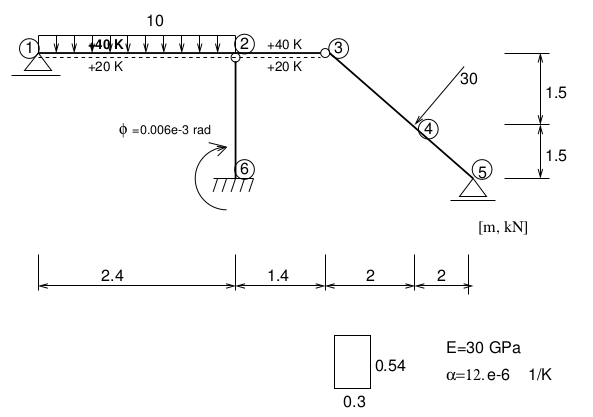
\includegraphics[scale=0.51]{pictures/chapter_oofem/structure_to_analyze.png}
\caption{Model strukture koju je potrebno analizirati. \cite{oofem-web}}
\label{fig:Structure_to_analyze}
\end{center}
\end{figure}

\lstinputlisting[language=python, label={code:oofem_input_file}, caption={Primjer datoteke ulaza za OOFEM}]{beam2d_1.in}


\section{Korištenje OOFEM alata iz Pythona}
\label{poglavlje:koristenje_pythona}
Nakon što smo opisali kako je OOFEM predviđen za korištenje, dajemo i nama najvažnije opis, kako koristiti OOFEM iz programskog jezika Python. U prvom poglavlju ukratko smo opisali što je metoda konačnih elemenata i kako ju koristiti, a u drugom pokazali smo kako koristiti OOFEM. Sada ćemo pokazati 2 načina na koje se može koristiti OOFEM iz Python-a. Prvi način koji nam nije pretjerano zanimljiv bazira se u potpunosti na načinu korištenja kao što se koristi i iz komandne linije putem učitavanja svih parametra iz datoteke ulaza. Onda rješavanje problema izgleda ovako:

\begin{lstlisting}[language=python, label={code:python_oofem_from_file}, caption={Pokretanje OOFEM alata pomoću Python-a i učitavanje ulaznih podataka iz datoteke}]
import liboofem

podaci = liboofem.OOFEMTXTDataReader("analiza_stapa_u_2d.in")
problem = liboofem.InstanciateProblem(podaci, liboofem.problemMode._processor, 0)
problem.checkProblemConsistency()
problem.setRenumberFlag()
problem.solveYourself()
problem.terminateAnalysis()
\end{lstlisting}

Prije nego što opišemo drugi način korištenja gdje se svi ulazni podaci konstruiraju pomoću Python objekata, ukratko ćemo opisati što je sve potrebno učiniti da bi mogli koristiti biblioteku \textit{liboofem}, kako je to omogućeno i što nam ona nudi. \par

Da bi se C++ kod mogao koristiti putem Python-a potrebno je zadovoljiti neke preduvjete. Pri tome postoji nekoliko načina, a autori OOFEM-a odlučili su se za korištenje Boost.Python biblioteke koja je dio boost C++ kolekcije. Boost je velik projekt koji sadrži više od 150 biblioteka i više od 23 milijuna linija koda za C++. Boost.Python je C++ bibliteka koja omogućuje besprijekornu interoperabilnost između C++-a i programskog jezika Python. Boost.Python omogućuje brz i lagan izvoz C++ koda u Python tako da se novonastalo sučelje gotovo ni ne mijenja u odnosu na C++ sučelje. Korištenjem Boost.Python biblioteke jedino potrebno za korištenje OOFEM-a jest definirati sve klase, metode i funkcije koje će se koristiti direktnim pozivanjem iz Python-a. To je učinjeno u datoteci \textit{oofemlib.cpp} koju se može pronaći na adresi \cite{oofemlib_source}. Datoteka s definicijama sadrži gotovo 2000 linija te definira Python biblioteku liboofem koju smo vidjeli u isječku koda \ref{code:python_oofem_from_file}. Važno je još reći da se prilikom kompiliranja OOFEM-a mora postaviti varijabu "USE\_PYTHON\_BINDINGS" na "ON" tako da se kompilira i datoteka \textit{oofemlib.cpp} te da se onda dobivena binarna datoteka \textit{liboofem.so} mora postaviti negdje gdje Python "gleda" module tako se liboofem može uključiti "importati" u Python. Više informacija o Boost.Python-u i generalno korištenju C++ koda u Python-u može se pronaći na \cite{boost_python}, \cite{ctypes} i \cite{swig}. \par

Nakon što smo opisali kako se kod napisan u C++-u uopće može koristiti u Python-u, opisati ćemo neke od mogućnosti koje nam \textit{liboofem} Python biblioteka daje te ćemo dati primjer kako je i koristiti. Kao što smo i opisali Boost.Python je omotač oko C++ koda stoga je glavna motivacija prijašnjeg (\ref{poglavlje:koristenje_oofema}) potpoglavlja bila upoznavanje mogućnosti OOFEM programa. Sada ćemo pokazati kako te iste funkcionalnosti koristiti iz Python-a, ali i neke dodatne mogućnosti koje nam samo Python okruženje nudi poput iteraktivnog ispitivanja pojedinih elemenata te grafički prikaz željenih vrijednosti. \par

Primjer kombinacije Python-ovih mogućnosti (točnije korištenjem matplotlib biblioteke) s mogućnostima OOFEM-a moguće je konstruirati mrežasti model i odmah ga i vizualizirati. Pokretanjem idućeg (\ref{code:python_oofem_matplotlib}) koda, dobiva se slika \ref{fig:visualization_of_oofem_mesh_grid_with_python}.

\begin{lstlisting}[language=python, label={code:python_oofem_matplotlib}, caption={Konstrukcija mrežastog modela i vizualizacija}]
from mpl_toolkits.mplot3d import Axes3D
from matplotlib import cm
import matplotlib.pyplot as plt
import numpy as np

import liboofem

# inicijalizacija uniformne mreze
mreza = liboofem.UniformGridField()

# postavljanje mreze na 2D geometriju
mreza.setGeometry(lo=(0,0),hi=(1,1),div=(2,2))

# mreza se proteze na 2x2 znaci da imamo 3x3 cvora, potrebno nam je 9 vrijednosti
mreza.setValues([-4, -3, -2, -1, 0, 1, 2, 3, 4])

# vizualizaciju zelimo na malo sirem podrucju
X,Y=np.meshgrid(np.arange(-.5,1.5,.1),np.arange(-.5,1.5,.1))

# funkcija koja vraca vektor vrijednosti u koordinatama
@np.vectorize
def vrijednost_na_koordinatama(x,y):
    return mreza.evaluateAtPos((x,y))[0]

Z = vrijednost_na_koordinatama(X,Y)

# vizualizacija pomocu matplotliba
fig = plt.figure()
ax = fig.gca(projection='3d')
surf = ax.plot_surface(X, Y, Z, linewidth=1, rstride=1, cstride=1,cmap=cm.coolwarm, shade=True)
plt.show()
\end{lstlisting}

\begin{figure}[h!t]
\begin{center}
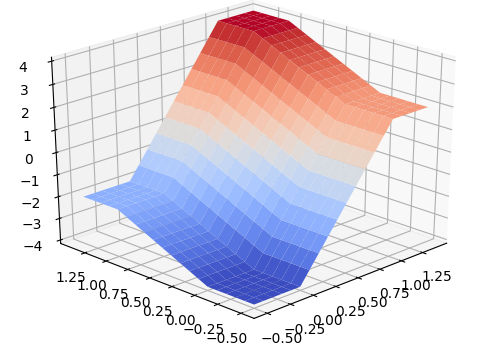
\includegraphics[scale=0.61]{pictures/chapter_oofem/liboofem_mesh_grid.png}
\caption{Vizualizacija uniformne pravokutne mreže konstruirane putem \textit{liboofem} biblioteke putem Pythona.}
\label{fig:visualization_of_oofem_mesh_grid_with_python}
\end{center}
\end{figure}

Sama mreža čvorova, kao i svi ostali elementi analize mogu se i individualno konstruirati što ćemo pokazati na idućem primjeru koda. Kod usko prati sve navedene korake iz prijašnjega potpoglavlja \ref{poglavlje:koristenje_oofema} što će biti jasno vidljivo, i modelira primjer sa slike \ref{fig:Structure_to_analyze} te je analogon ulaznoj datoteci \ref{code:oofem_input_file} za analizu pomoću OOFEM-a putem komandne linije. Nakon same analize moguće je, kao i u prošlom primjeru konstruirati razne vizualizacije što prepuštamo čitateljima radi toga da sam kod bude što čišći i relevantniji samoj zadaći koja je opisivanje korištenja \textit{liboofem-a} radi analize konačnih elemenata.

\lstinputlisting[language=python, label={code:python_oofem_full_example}, caption={Korištenje OOFEM putem Python-ovog sučelja}]{uredeni_primjer.py}

Važno je još napomenuti da omotač oko C++ koda programa OOFEM ne obuhvaća sve moguće značajke u jednakom obimu. Tako primjerice iz gornjeg koda vidjeli smo da se može koristiti konačni element greda u dvodimenizionalnom prostoru (\textit{liboofem.beam2d}), ali radi lakšeg prototipiranja i bolje apstrakcije koda ostali konačni elementi nisu tako definirani. Definiciju \textit{beam2d} konačnog elementa može se pronaći u datoteci \textit{oofemlib.cpp} na adresi \cite{oofemlib_source} između 1544-te i 1585-e linije koji izgleda ovako:

\begin{lstlisting}[caption={Implementacija omotača oko generalnog konačnog elementa i specifičnog konačnog elementa \textit{beam2d}}]
/*****************************************************
* Element
*****************************************************/
// element(aClass,domain=defaultDomain,**kw)
object element(bp::tuple args, bp::dict kw)
{
    // extracts first python argument (string element type)
    string aClass = extract<string>(args[0])();
    // extracts values from args if they are specified
    int number =     len(args)>1? extract<int>(args[1])() : 0;
    Domain *domain = len(args)>2? extract<Domain*>(args[2])() : nullptr;
    /* ????????????????
    // if no material is specified, set it to 1
    if (!kw.has_key("mat")) { kw["mat"] = 1; }
    // if no cross section is specified, set it to 1
    if (!kw.has_key("crosssect")) { kw["crosssect"] = 1; }
    // if no domain is specified and one already exists in the script, use that one
    if (domain == nullptr && temp_global.has_key("defaultDomain")) { domain = extract<Domain*>(temp_global["defaultDomain"])(); }
    if (domain==nullptr) { LOG_ERROR(oofem_errLogger,"wrong Domain"); }
    ???????????????????? */
    // create Element (convert aClass to char* - expected by classFactory.createElement)
    auto elem = classFactory.createElement(aClass.c_str(),number,domain);
    // if elem==nullptr, something was wrong
    if (!elem) { OOFEM_LOG_ERROR("element: wrong input data"); }
    // sets globalNumber == number befor initializeFrom
    elem->setGlobalNumber(number);
    // construct OOFEMTXTInputRecord from bp::dict **kw
    OOFEMTXTInputRecord ir = makeOOFEMTXTInputRecordFrom(kw);
    // pass input record to elem
    elem->initializeFrom(&ir);
    // convert element to PyObject (expected by raw_function, which enables fun(*args,**kw) syntax in python)
    return object(ptr(elem.release()));
}

// auxiliary constructor for specific element type (name is passed as first argument)
object createElementOfType(const char* type, bp::tuple args, bp::dict kw)
{
    args = len(args)>1? bp::make_tuple(type,args[0],args[1]) : len(args)>0? bp::make_tuple(type,args[0]) : bp::make_tuple(type);
    return element(args, kw);
}
// specific elements
object beam2d(bp::tuple args, bp::dict kw) { return createElementOfType("beam2d",args,kw); }

...

BOOST_PYTHON_MODULE (liboofem)
{

...

    def("element", raw_function(element,1));
    def("beam2d", raw_function(beam2d,0));

...

}
\end{lstlisting}

Iz koda je vidljivo da se korisnicima ostavlja mogućnost korištenja svih konačnih elemenata OOFEM-a, ali kroz malo drugačije sučelje. Tako se primjerice za konstrukcija za ostale konačne elemente odvija na idući način:

\begin{lstlisting}[language=python, caption={Primjer konstrukcije konačnih elemenata koji nemaju implementiran direktan poziv}]
greda_direktno = liboofem.beam2d(1, domain, nodes=(1,2), ...)
greda_indirektno = liboofem.element('beam2d', 1, domain, nodes=(1,2), ...)
greda_indirektno2 = liboofem.InputRecord(1, "beam2d", {"nodes": (1,2), ...})
stap_indirektno = liboofem.element('truss2d', 1, domain, nodes=(1,2), ...)
\end{lstlisting}

Osim za konačne elemente, identičan postupak se odvija i za ostale komponente koje nasljeđuju klasu \textit{FEMComponent} opisanu u potpoglavlju \ref{poglavlje:struktura_koda} i prikazanu na slici \ref{fig:FEMComponent_inheritance} poput materijala (\textit{Material}), poprečnih presjeka (\textit{CrossSection}), vremenskih funkcija itd. \par

U ovom dijelu prikazali smo više načina korištenja OOFEM-a putem Python-a te nekoliko ideja za nadogradnju što se još može postići. Pokazali smo kako je i gdje implementiran omotač oko C++ koda te kako i gdje u slučaju potrebe i želje treba definirati dodatne metode koje trenutno nisu podržane za interakciju kroz Python. U posljednjem poglavlju pokazujemo još jednom kako koristiti OOFEM i \textit{liboofem} biblioteku za Python za analizu metode konačnih elemenata.


\section{Vizualizacija rezultata}
OOFEM pruža nekoliko načina kako dobivene rezultate prikazati. Opisat ćemo 3 različita načina i dati nekoliko primjera kako te vizualizacije izgledaju.
\begin{enumerate}
    \item OOFEG - OOFEM izvorni kod dolazi s OOFEG, X-windows baziranim vizualizacijskim alatom. Kako je baziran na X-windows bibliotekama više manje upotreba mu je ograničena na unix platforme. OOFEG je razvijen pomoću Elixir i Ckit biblioteka koje više nisu aktualne stoga se grafičko sučelje izgleda kao "zamrznuto" u vremenu kasnih 90-tih i daljnji razvoj više nije lako ostvariv. OOFEM je isto limitiran u mogućnostima 3D vizualizacije. Radi svega toga OOFEG je uredu za upotrebu kod relativno jednostavnih primjera ali ubrzo postaje nedovoljno moćan. OOFEG ima jedan dobar slučaj upotrebe, a to je za vizualizaciju mreže te se nakon što su instalirane sve njegove potrebne komponente koristi s \textit{oofeg -f ulazna\_datoteka.in}. 
        \begin{figure}[h!t]
        \begin{center}
        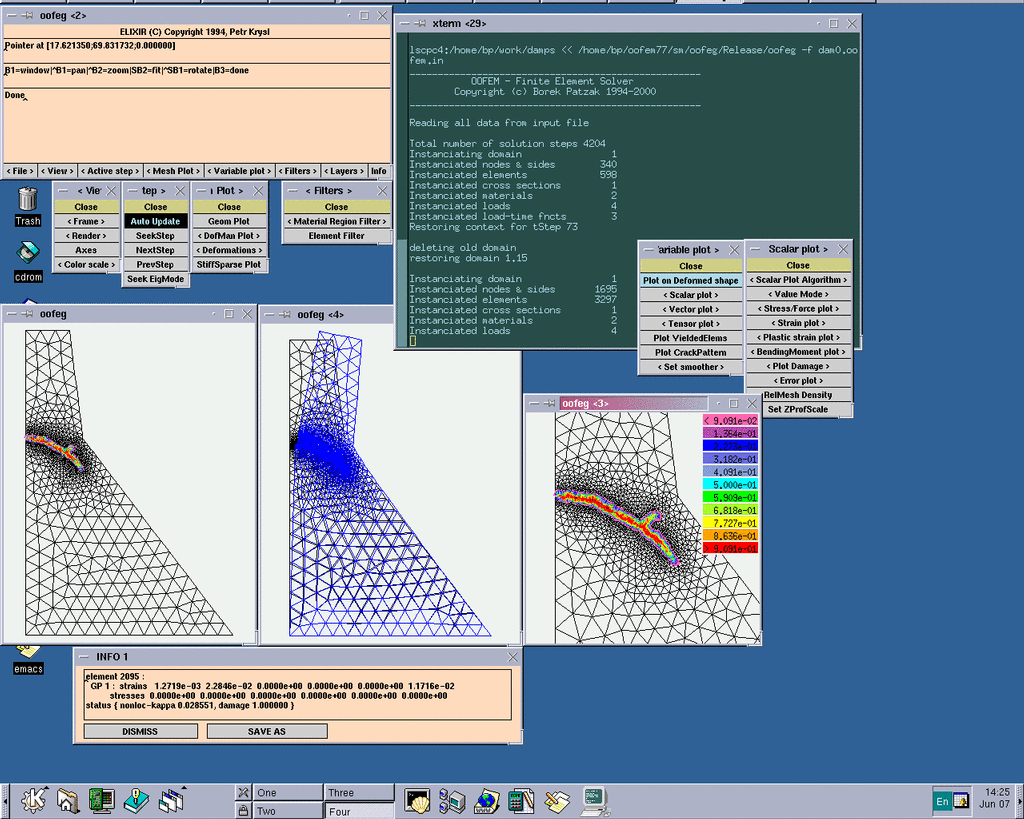
\includegraphics[scale=0.3]{pictures/chapter_oofem/oofeg_koyna_dam.png}
        \caption{Vizualizacija pomoću OOFEG grafičkog procesora. \cite{oofem-web}}
        \label{fig:oofeg_example}
        \end{center}
        \end{figure}
    \item ParaView - OOFEM omogućava na jednostavan način pretvorbu izlazni podataka u VTK format što omogućava vizualizaciju putem softvera treće strane poput ParaView-a i MayaVi-a. Dobra strana toga je to što su takvi alati specijalizirani za vizualizaciju te omogućuje znatno više značajki te se u odnosu na OOFEG i dalje razvijaju i napreduju. Kao što smo naveli u potpoglavlju \ref{poglavlje:koristenje_oofema} pod rednim brojem četiri, za izvoz podataka u VTK format dovoljno je dodati jednu liniju. Jednako tako dodavanje samo jedne linije u Python kod rezultati će se ispisati u datoteku i u VTK formatu. Nakon završetka analize, konstruirati će se datoteke s informacijama za svaki korak koje se uvezu u našem slučaju u ParaView. Nadalje, za uvesti podatke u ParaView potrebno je samo označiti datoteku koja ima ekstenziju \textit{.pvd} i koja ima zapisane putanje do datoteka s podacima o rezultatima analize. Na slici \ref{fig:paraview_example} dajemo primjer strukture vizualizirane pomoću ParaView softvera.
        \begin{figure}[h!t]
        \begin{center}
        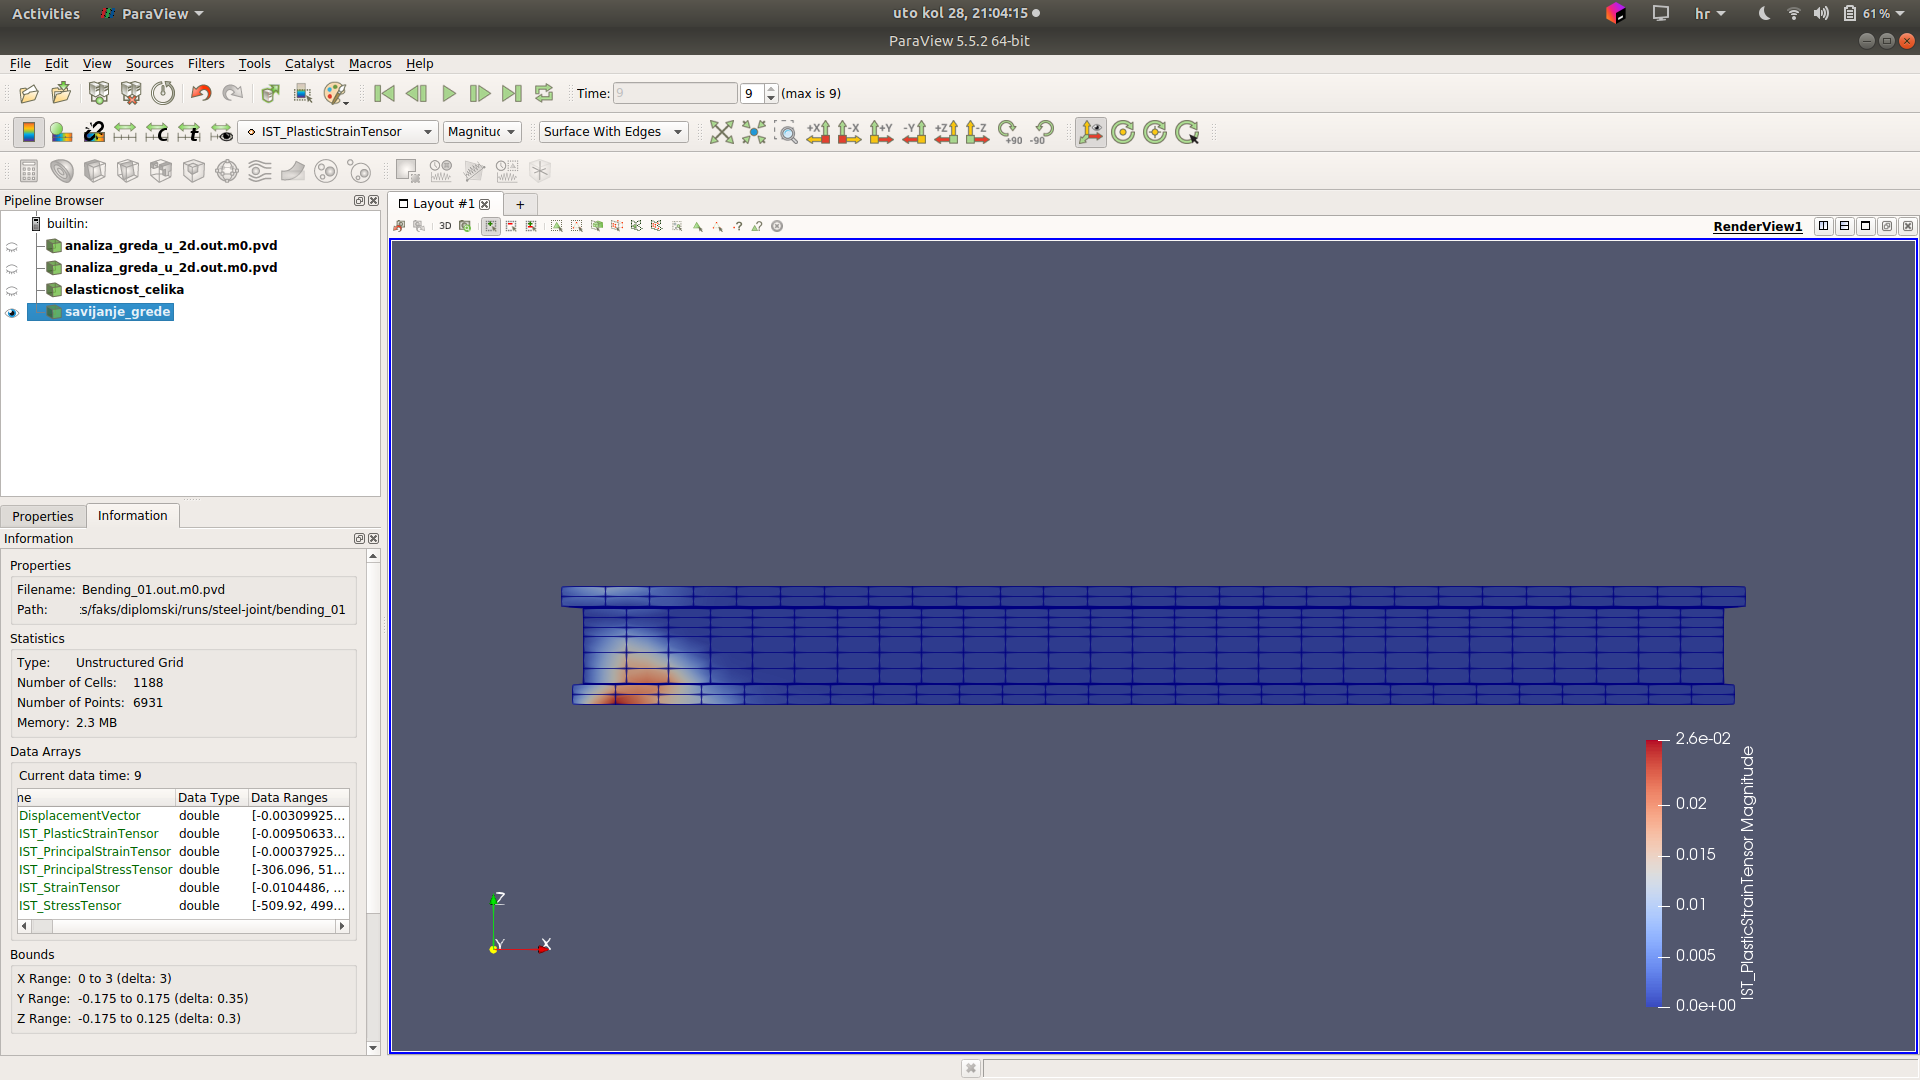
\includegraphics[scale=0.2]{pictures/chapter_oofem/paraview_beam_bending_full.png}
        \caption{Vizualizacija grede na koju se vrši pritisak pomoću ParaView softvera.}
        \label{fig:paraview_example}
        \end{center}
        \end{figure}
    \item Python - Kao što smo pokazali na gornjem primjeru, ekosustav Python-a dolazi s velikom količinom alata koji nam mogu pomoći u vizualizaciji bilo kakvih podataka. Tako smo na slici \ref{fig:visualization_of_oofem_mesh_grid_with_python} prikazali mrežu konačnih elemenata konstruiranih pomoću OOFEM-a. Jedna od bitnijih biblioteka za vizualizaciju je \textit{matplotlib} o kojoj se više može pronaći na web stranici \cite{matplotlib_web}.
\end{enumerate}

Iz svega navedenoga preporuka za vizualizaciju jest koristiti već postojeće alate pomoću jednostavne funkcije izvoza rješenja, te u slučaju potrebe za nekom dodatnom vizualizacijom koja obuhvaća nešto što se iz uobičajenih rezultata ne dobije poput matrice krutosti pojedinih elemenata koristiti Python-ov ekosustav koji pruža dobru podršku za proizvoljne posebne slučajeve.

\chapter{Testni primjer}
U ovom poglavlju pokazati ćemo kako riješiti zadatak \ref{fig:problem__not_noted} koji smo ručno riješili u poglavlju \ref{primjer_zadatka_i_rjesenja}. Zadatak ćemo riješiti na 3 načina pomoću OOFEM-a te usporediti rezultate u odnosu na ručno rješavanje. Prvo ćemo sastaviti datoteku ulaza s potpunim problemom te pokrenuti OOFEM s njome. Za drugi način koristiti ćemo Python i pomoću njega učitati ulaznu datoteku koju smo koristili i u prvom načinu. Za treći način rješavanja u potpunosti ćemo definirati ulazne podatke u Python-u i dobiti rješenje. Za vizualizaciju rješenja koristiti ćemo ParaView i vizualizaciju pomoću Python-a.

\section{Rješavanje učitavanje datoteke u OOFEM putem terminala}







\section{Problem}
p

\section{Generiranje ulaznih podataka}
p

\section{Rješavanje problema}
r

\section{Vizualizacija dobivenih rezultata}
v









\chapter[Naslov poglavlja u sadržaju][Kratki naslov poglavlja]{Naslov poglavlja}	
% ukoliko naslov nije jako dugacak dovoljno je samo \chapter{Naslov poglavlja} 

\section[Naslov sekcije u sadržaju][Kratki naslov sekcije]{Naslov sekcije}
\subsection{Naslov podsekcije}
\begin{thm}
Iskaz teorema u kojem se javljaju skupovi  $\N$, $\Z$, $\Q$, $\R$ i $\C$.
\end{thm}
\begin{conj}
Iskaz slutnje u kojoj se javljaju funkcije $\tg$, $\tgh$ i $\sh$.
\end{conj}
\begin{cor}
Iskaz posljedice u kojoj se javljaju skupovi $\Ker T$ i $\slika T$..
\end{cor}
\begin{proof}
Dokaz posljedice se nalazi u \cite{kljuc}. Pogledajte i \cite{kurepa1956convex}, \cite{kurepa1981funkcionalna} te \cite{Dutkay:2009}.
\end{proof}
jsfdsqF
SG
SFG
FSG
DF
GS
FG
SFG
SFG

SFG

SG
SDFG
SF
GS

DG
 SD
S


SD
 

DFGSDFG


SDGSDF


SDGSDGF


SDGFSFDG


SDGSDG  sdfsfg f fdh fgj gh jgjk jkj k yk k klk l fs fd gsdfg dfh dfghj fj ghjk gjk jlk sdf 
$x_1+x_2+x_3+x_4=12$ $x_1+x_2+x_3+x_4=12$
 $x_1+x_2+x_3+x_4=12$ $x_1+x_2+x_3+x_4=12$ $x_1+x_2+x_3+x_4=12$ $x_1+x_2+x_3+x_4=12$
 $x_1+x_2+x_3+x_4=12$ $x_1+x_2+x_3+x_4=12$ $x_1+x_2+x_3+x_4=12$
$x_1+x_2+x_3+x_4=12$ 
SDGSG sdfsfg f fdh fgj gh jgjk jkj k yk k klk l fs fd gsdfg dfh dfghj fj ghjk gjk jlk sdf sfdh j fj tuk ugad h j yrtu iru i
\[ z \left( 1 \ +\ \sqrt{\omega_{i+1} + \zeta -\frac{x+1}{\Theta +1} y + 1}
\ \right) =  1 \]

GSDFGSDFG



\begin{equation}
\label{eq:jed111}
	1+1=2
\end{equation}

SDG
SDFGS

SDFGSFG


SFGSFG


SDFGSFG


SDGSFG

\label{stranica}
Na stranici \pageref{stranica} se nalaza slika u \textbf{png} formatu.
% slike smiju biti u svim formatima koje podrzava pdf (pdf, jpg, png)
\begin{figure}[h!t]
\begin{center}

\includegraphics[scale=0.5]{mosaic-from-pompeii.png}
\caption{Prva slika}
\end{center}
\end{figure}

Na slici \ref{fig:3d} se nalazi 3D graf neke funkcije. 

\begin{figure}[h!t]
\centering 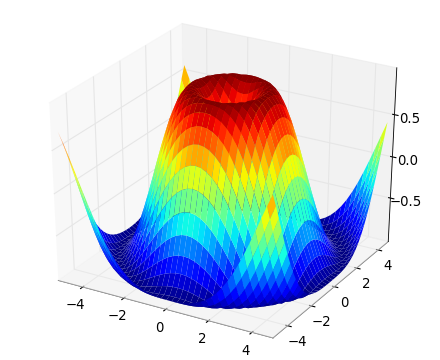
\includegraphics{surface3d.png}
\caption{Druga slika}
\label{fig:3d}
\end{figure}

kao i jedna vrlo komplicirana formula koja slijedi iz \eqref{eq:jed111}
\[ \sum_{i=1}^{\infty}A_{x_1}\times A_{{\alpha}_2}\oslash\iint_{\Omega}x^2\ddagger\limsup_{n\in\N}\frac{\alpha+\theta+\gamma}{n^{\omega}}\;\;\text{je u stvari}\;\;\biguplus_{r\in\Q}\overline{\Xi_i \mathop\Theta_{\substack{j\in\C \\ j\ni i\Q}} \Upsilon^{k^j} \underset{\ast}{\Psi} \hslash\vert_{\{\alpha\}}}.\]

% Na kraju diplomkog rada stavlja se  bibliografija
% Najprije definiramo nacin prikazivanja bibliografije, u ovom slucaju verzija amsplain stila
\bibliographystyle{babamspl} % babamspl ili babplain

% U datoteku diplomski.bib se stavljaju bibliografske reference
% Bibliografske reference u bib formatu se mogu dobiti iz MathSciNet baze, Google Scholara, ArXiva, ...
\bibliography{diplomski}

\pagestyle{empty} % ne zelimo brojanje sljedecih stranica

% I na koncu idu sazeci na hrvatskom i engleskom

\begin{sazetak}
Metoda konačnih elemenata je jedna od važnijih numeričkih metoda za rješavanje problema u inženjerstvu poput strukturne analize objekata. Korisnost metode može sve vidjeti po količini alata koji su razvijeni za nju te po tome što je standard u industrijama poput zrakoplovne i automobilske. Cilj ovog diplomskog rada bio je predstaviti OOFEM (Object Oriented Finite Element Method), jedan takav alat i strukturu njegovog otvorenog koda tako da se budući korisnici mogu lakše snaći u njegovom korištenju, a posebice ako im se ukaže potreba za nadogradnjom i implementacijom novih funkcionalnosti. U opisu OOFEM-a poseban naglasak stavljen je na strukturnu analizu te konačne elemente i materijale potrebne poput greda i šipki u dvodimenzionalnom sustavu analize. Središnji je dio rada opis korištenja OOFEM-a putem njegovog sučelja za korištenje iz programskog jezika Python.
Osim generalnih informacija što se sve i kako može koristiti putem Python-a, priloženo je i nekoliko primjera te je čak i ukratko opisan postupak kako je izrađeno sučelje iz C++-a tako da se može koristiti u Python-u. Motivacija iza toga je ta što nisu sve značajke izložene putem Python sučelja, te se ukratko pokazuje kako bi se mogle izložiti nove funkcionalnosti u slučaju potrebe.
\end{sazetak}

\begin{summary}
The finite element method is one of the most important numerical methods for solving engineering problems such as structural analysis of objects. The usefulness of the method can be seen by the amount of tools developed for it and by the fact that it became standard in industries such as aviation and automotive. The aim of this thesis was to present OOFEM (Object Oriented Finite Element Method), enabling future users to use it more easily, especially if they need to upgrade existing or implement new functionalities. In the description of OOFEM, a special emphasis was placed on the structural analysis method and finite elements and materials needed for it as beams and trusses in two-dimensional analysis. The central part of the thesis describes the use of OOFEM through its interface for use in the Python programming language. In addition to general information about what and how to use it through Python, a few examples are included, and a brief description of how a C++ interface is made so that it can be used in Python. The motivation behind it is that not all features are exposed through Python interfaces, so there is brief introduction how new functionalities could be exposed if necessary.
\end{summary}

% te zivotopis

\begin{cv}
Ivan Laković rođen 14. studenog 1993. godine u Puli. Završava osnovnu školu u Svetom Lovreču, a zatim i opću gimnaziju u Pazinu. Na Matematičkom odsjeku Prirodoslovno-matematičkog fakulteta Sveučilišta u Zagrebu 2012. godine upisuje preddiplomski studij matematike. Izobrazbu nastavlja na istom fakultetu, na diplomskom studiju Računarstvo i matematika. Jedan semestar studija provodi na razmjeni na Sveučilištu u Wroclawu (Uniwersytet Wrocławski, Instytut Informatyki) Za trajanja studija, osim studiranja natječe se i postiže dobre rezultate na studentskim natjecanjima \textit{Mozgalo, Airtravel Hackaton, AI Battleground, Try$\{$code$\}$catch i tehnološkoj areni STEM games-a} te pohađa i kolegij na Raspodjeljeni razvoj programske potpore (Distributed software development) koje se održava na FER-u u suradnji sa sveučilištima Mälardalen University u Švedskoj i Politecnico di Milano u Italiji. Diplomski studiji završava 2018. godine pod mentorstvom prof.dr.sc. Luke Grubišića.
\end{cv}

\end{document}